%!TEX program = xelatex

\documentclass[lang=cn,headings=optiontohead]{elegantpaper}

\title{Libra 监管与合规白皮书}

\author{胡大鹏、周子涵、赵旭初、孔德云、李炼炫、黄小雁\thanks{本文所有作者就职于 OK 区块链工程院研究部,联系方式: dapeng.hu@okcoin.net}}

\institute{OK区块链工程院}

%\version{Draft: 0.3}

%\date{\today}

\begin{document}

\maketitle

%----------------------------------------------------------------------------------------
%	论文摘要
%----------------------------------------------------------------------------------------
\begin{abstract}
Libra 的愿景之一是利用分布式账本技术构建全球化的金融基础设施。要求 Libra 网络满足了解客户(KYC), 反洗钱(AML)、反恐怖主义融资(CFT)等金融监管与合规要求。
本文阐述了 Libra 关于金融监管与合规的相关架构设计。首先我们指出:分布式账本技术必须与金融市场基础设施原则(PFMI)相结合,才能构建能实际应用的金融系统;其次,我们提出了账本数据的完整性、公开性、隐私性三角不可能原理。由此得出结论:分布式账本必须与链下的身份管理、合规审核系统集成,才能满足监管与合规的需求。再次,我们总结了加拿大央行、欧洲央行、日本央行等相关工作的经验。最后,从组织安排、账本数据结构、准入与账本体系、合规协议4个方面阐述了合规框架设计。


\end{abstract}


%\tableofcontents

%\lstlistoflistings

%\newpage
%----------------------------------------------------------------------------------------
%	Section 1: 简介
%----------------------------------------------------------------------------------------
\section{介绍}

金融市场基础设施(FMI)是由多个彼此独立的参与机构形成的多边系统,
有助于支付、证券、衍生品合约等货币和其它金融交易的清算、结算和记录。
它是金融运行的的基础,是金融经济系统高效、安全运行的重要保证。
对于畅通货币政策传导机制、加速社会资金周转、优化社会资源配置、维护金融稳定并促进经济增长有重要意义。

现代金融市场基础设施虽然在不同国家有不同的具体组织形式,但一般包含以下五种基本职能及对应的支撑机构:

\begin{itemize}
    \item [\dag] \textbf{支付功能}:支付系统(Payment System,PS) 提供资金转账服务。
    \item [\dag] \textbf{存管功能}:中央证券存管(Central Securities Depository ,CSD) 提供证券集中登记、托管、赎回等服务。
    \item [\dag] \textbf{清算功能}:中央对手方(Central Counter Party ,CCP) 作为一种清算机制,清算机构自身介入已经达成的交易,成为卖方的买方和买方的卖方,确保已达成交易正常履约,是防范金融市场系统性风险的重要手段。
    \item [\dag] \textbf{结算功能}:证券结算系统(Securities Settlement system,SSS) 提供证券过户和结算服务(如典型的券款对付DvP)。
    \item [\dag] \textbf{报告功能}:交易数据库(Trade Repository ,TR)是为增强市场透明性而集中收集、保存并向监管和公众披露各类交易数据的机构,是金融危机后为加强场外衍生品市场监管而新出现的FMI类型。
\end{itemize}

现代金融市场基础设施为全球金融市场交易提供了一个相对稳定、可靠的基础和环境。但仍然存在一定局限: 
\begin{enumerate}
    \item 今天的金融市场由众多不同层级的参与者组成,并形成了一个复杂的网络,其业务流程和相关技术系统也非常复杂,同时许多手工处理步骤依然存在。
    \item 每一个参与者需要保存和维护自己独立、专有的数据库,每一交易数据的变化需要通知利益相关者并需要在不同系统之间进行对账并保持一致。
    \item 交易以及清算,结算和抵押品管理等系统,在不同历史时期为了不同的需要而建立,没有广泛接受的标准,系统之间缺乏互操作性。
\end{enumerate}
金融市场基础设施的这些局限,不仅使结算周期变长、增加后台处理成本,也增加了整个金融市场的风险。
2008年金融危机爆发以来,国际社会对引起危机的根源进行了深刻反思,结论之一就是要加强安全、高效、透明、规范的金融市场基础设施建设。
分布式账本作为一种新的账本管理技术,非常有潜力改善现有金融市场基础设施的局限性。
它与传统中心化、层级化的交易处理和记账方式截然不同。
分布式账本的去中心化特性,可以消除一些金融市场中间环节、实现点对点直接交易,从而简化业务流程,缩短交易周期,有效降低风险、提高效率、节约成本。

Libra 的使命之一是基于分布式账本技术,建立一套通用的、无国界的、为数十亿人服务的金融市场基础设施,创造一个更加普惠的金融体系。
金融是一个强监管的行业,金融市场基础设施在金融的监管体系中扮演了关键的角色,它们为金融市场制定了统一的流程、规则;
而且监管层可以通过它们监管整个金融系统。
下图是美国金融监管架构\footnote{源自芝加哥联邦储备银行:\url{https://www.chicagofed.org/markets/view-lasalle-street/us-reg-authority}},从中可以看到基础设施在金融监管方面的重要作用。

\begin{figure}[h!]
    \centering
    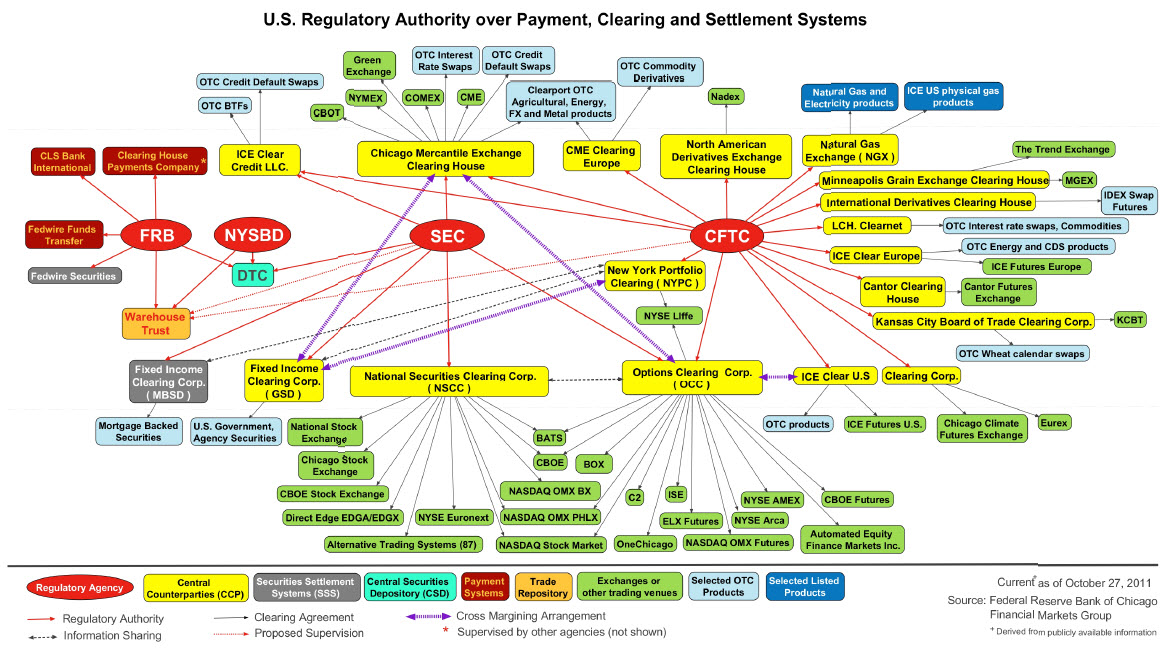
\includegraphics[width=12cm, keepaspectratio]{images/regulatory-over-PCS.jpg}
    \caption{美国联邦金融监管架构}
    \label{fig:USAReg}
\end{figure}

%基于上述这些基础设施服务机构,其它金融机构,如交易场所(交易所或场外市场)、证券发行方、托管银行、买方/卖方、经纪商、清算会员、结算代理行等,面向用户展开各种金融服务。它们共同形成了一个多层级的、互相协作、互相制约的复杂网络。

我们认识到,Libra 必须要满足金融监管与合规的需求,才能成为安全、高效、规范、可大规模应用的金融市场基础设施。
在7月16与17日举行的听证会上,美国参众两院也对 Libra 提出了一些列关于金融监管与合规的要求。
作为回应,此白皮书将介绍 Libra 网络在了解客户(KYC), 反洗钱(AML)、反恐怖主义融资(CFT)等方面的解决方案。

本文的结构如下:
\begin{itemize}
    \item[] 第2节:介绍分布式账本技术(DLT)与金融市场基础设施原则(PFMI)的关系。
    \item[] 第3节:介绍账本管理的三元悖论,解释分布式账本固有的抗审查性。
    \item[] 第4节:介绍加拿大央行、欧洲央行、日本央行、新加坡金融管理局的相关工作和结论。
    \item[] 第5节:介绍记账权与审核权分离模式下的组织安排,矿工与合规机构的协作关系。
    \item[] 第6节:介绍与合规相关的账本数据结构,支持与链下的身份管理系统集成。
    \item[] 第7节:介绍分层的账户体系结构与准入机制。
    \item[] 第8节:介绍交易前置的合规验证协议,与链下的反洗钱等合规系统集成。
\end{itemize}

%\begin{figure}[h!]
%    \centering
%    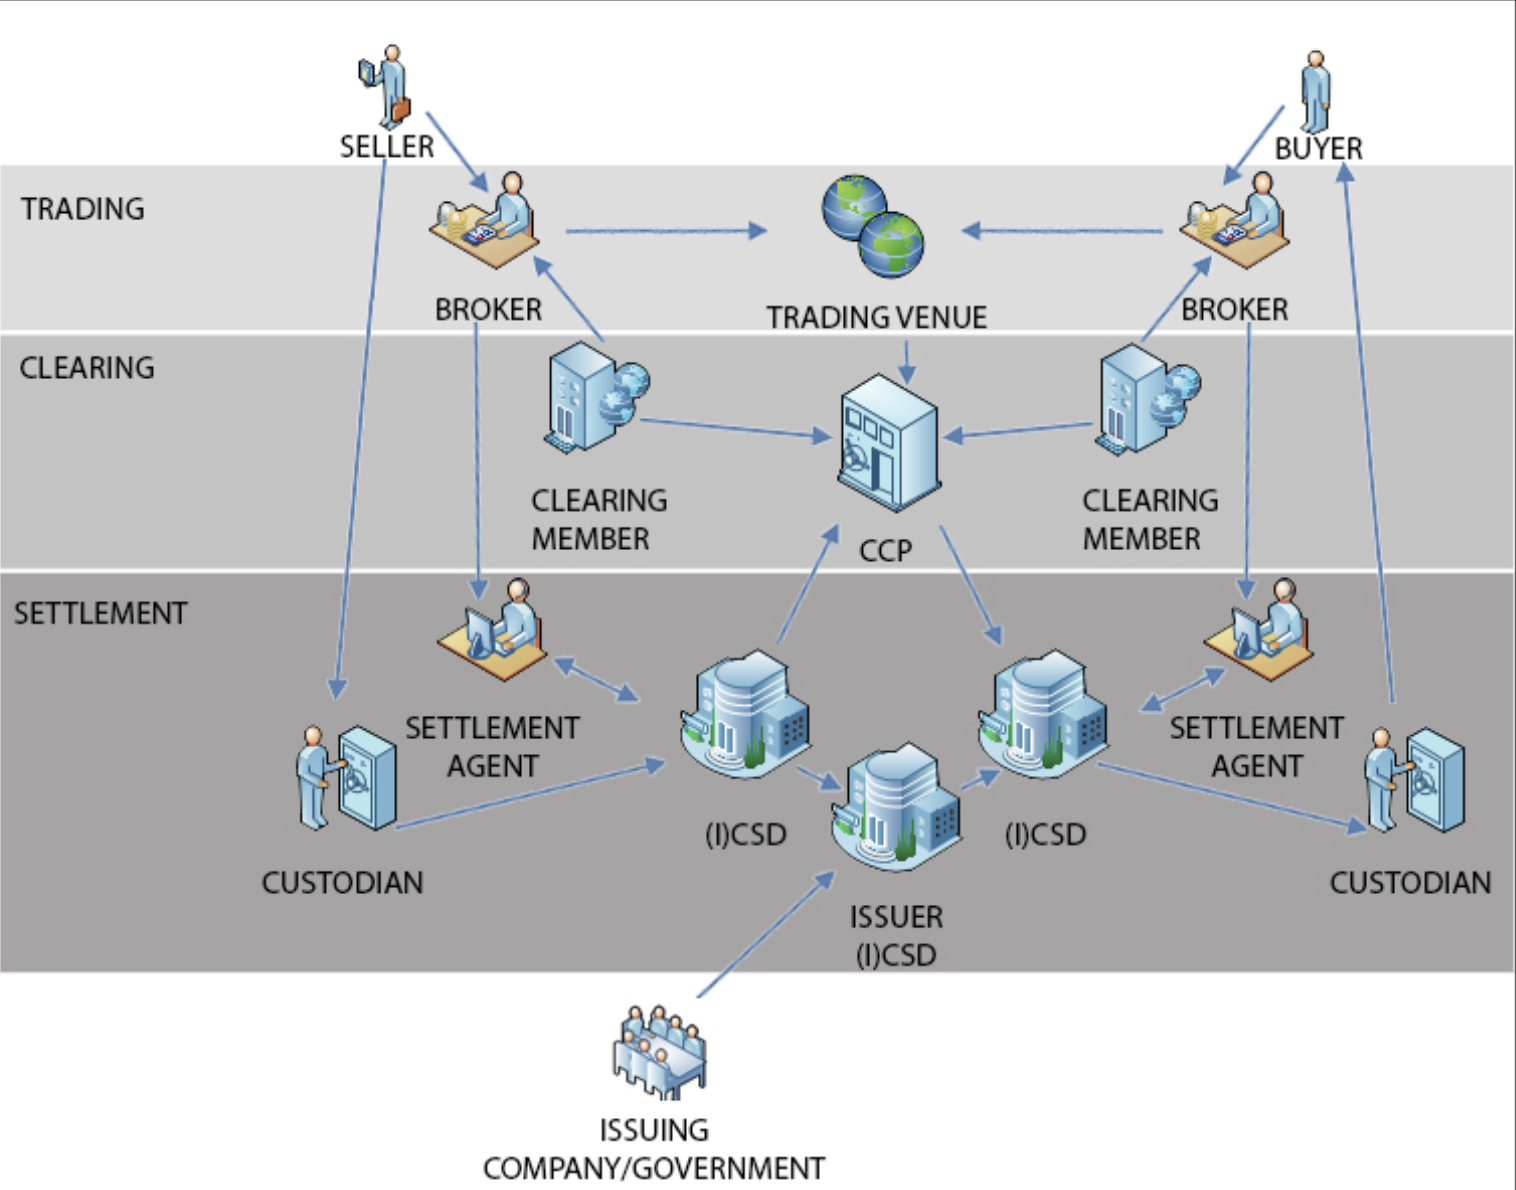
\includegraphics[width=8cm, keepaspectratio]{images/Security-Arch.png}
%    \caption{证券金融基础设施}
%    \label{fig:security}
%\end{figure}





%----------------------------------------------------------------------------------------
%	Section 2: 金融危机的反思
%----------------------------------------------------------------------------------------
\section{金融市场基础设施原则与分布式账本}\label{sec:pfmi}

2008年金融危机爆发以来,国际社会对于构建安全、高效的金融基础设施提出了更高的要求。十多年来诞生了两方面的成果。

一个是2012年4月国际清算银行(BIS)发布的《金融市场基础设施原则》(PFMI)\cite{pfmi}。
针对金融市场基础设施的建设,PFMI分析了金融系统的主要风险(系统性风险、法律风险、流动性风险、业务风险、托管与投资风险、运营风险),
从9个方面(总体架构、信用与流动性风险管理、结算、证券存管与交易、违约管理、运营风险管理、准入机制、效率、透明度)提出了24条指导原则。
PFMI从金融系统顶层设计的角度,进一步确立了全球金融市场基础设施建设标准,为世界各国开展相关工作指明了方向。

另一个是以比特币为代表的分布式账本技术。
在2008年,中本聪(Satoshi Nakamoto)发表了比特币的白皮书,描述了一种不依赖于单一信用机构的记账技术。
这种后来被称为分布式账本的新技术迅速发展,各种数字货币与公有链竞相出现,构建了一个全新的金融服务生态,引起国际社会特别是金融界的广泛关注和高度重视。
分布式账本提供了公共的账本管理平台,互相独立的金融机构可以在同一个账本上彼此协作。
这种公共账本模式为对金融系统的深远影响体现在以下几个方面:

\begin{enumerate}
    \item 效率:跨行、跨境交易可以在公共账本上一次性完成结算,缩短了交易环节,简化了交易流程,降低了交易摩擦。
    \item 风险:由于缩短了中间转账的环节,降低了对于中间人的信用风险、流动性等风险。
    \item 透明度:资金流数据集中记录在一个公开、透明的账本上,提高了交易数据的完整性和可访问性。相对于监管多个分散的账本,监管一个公共账本会大幅降低监管的难度。无论是对于监管层、还是金融机构来讲,监管合规的成本也会大幅降低。
    \item 自动化:利用智能合约,将金融资产映射为可编程的Token,提高资产发行、销售、流转、托管等业务的电子化、自动化
    \item 标准化:众多金融机构使用同一个账本,便于统一彼此之间的通信协议、数据格式,提高金融行业规范化、标准化程度
    \item 全球化:分布式账本建立在全球化的互联网基础上,而不是封闭的专用金融网络。各个国家和地区可以共享同一套系统,便于搭建国际化的金融系统。
    \item 避免重复建设:采用国际化的公共账本,对于金融机构,可以减轻维护独立账本的负担;对于国家和地区,缓解了各自建设金融专用网络的需求。
\end{enumerate}

总之,对重塑金融业未来发展,PFMI和分布式账本都有重大的价值。
PFMI 是自顶向下、为金融系统的顶层设计提供了指导原则;分布式账本是自底向上、在全新的账本管理技术的基础上,重构整个金融系统。
PFMI与分布式账本技术的出现有相同的时代背景,都是源自于次贷危机的影响,它们的目标都是要建立更加安全、高效、可靠、可信的金融系统。
这二者虽然方法和方式不同,但是同源同宗,本质上是互补的。



%----------------------------------------------------------------------------------------
%	Section 3: 挑战
%----------------------------------------------------------------------------------------
\section{账本管理的三元悖论}\label{sec:triangle}
根据PFMI的指导原则,金融基础设施应该接受中央银行、市场监管者或者其它管理部门适当、有效的管理、监管和监督。
为了保证金融系统的安全和稳定,各国央行和监管机构对金融机构提出了Know-Your-Customer(KYC)、Anti-Money-Laundering(AML)、Counter-Financing-of-Terrorism (CFT)等合规要求。
但是在实际应用过程中,分布式账本技术在这方面一直比较弱,甚至有些产品的设计目标就是抗审查、抗监管。
从一定程度上助长了洗钱等金融犯罪行为。
根据日本警方报告\cite{jp_report},2018年加密货币洗钱案件增加了十倍。
2017年,日本国家警察局发现了不到700起加密洗钱事件;2018年,他们发现了7,000多起同类案件。

%分布式账本要成为金融基础设施,在保留其技术优势的同时,还要满足金融监管的要求。
分布式账本固有的抗审查性可以用一个三元悖论来解释:

\begin{quotation}
    \textbf{任何独立的账本管理系统只能同时实现以下三个目标中的两个: 去中心化账本管理、账本数据的完整性、账本数据的隐私性。}
\end{quotation}

\begin{figure}[h!]
    \centering
    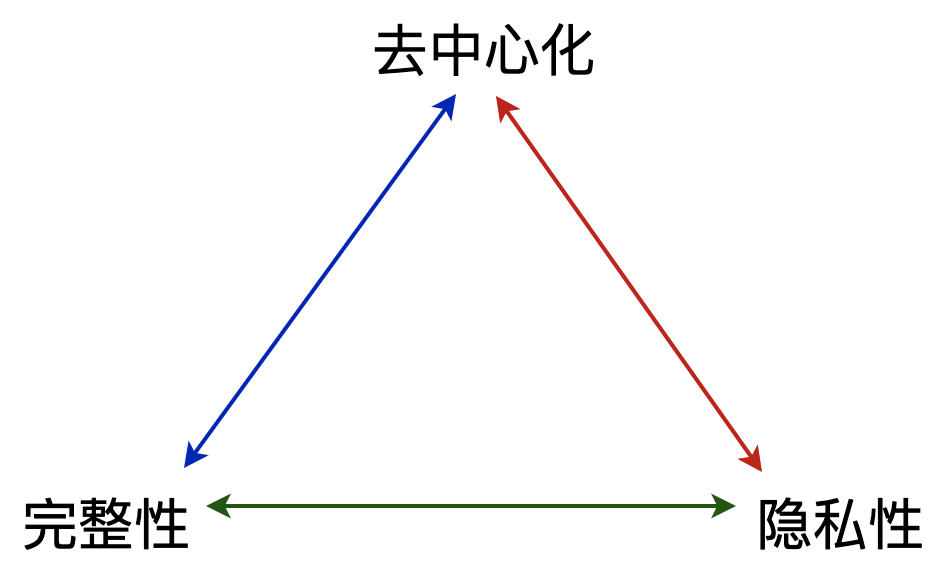
\includegraphics[width=9cm, keepaspectratio]{images/triangle.png}
    \caption{账本数据的三元悖论}
    \label{fig:triangle}
\end{figure}

%这个矛盾的根源在于分布式账本作为共享账本,满足了账本数据的公开性,无法再满足完备性。
%一般来讲,在金融系统中,无论是中心化账本还是去中心化账本,都无法同时满足公开性和完整性。

其中去中心化、完整性、和隐私性的定义如下:
\begin{itemize}
    \item[\dag] \textbf{去中心化}:
    账本数据保存在多个不同的节点中,便于其它节点验证账本数据,并且保证账本的可信度。

    \item[\dag] \textbf{完整性}:
    按照PFMI的需求:金融机构或者金融监管方需要完整的账户信息和交易信息、以及其它用于验证交易是否合规的相关信息。
    
    \item[\dag] \textbf{隐私性}:
    只有交易的参与方与金融监管方才能了解交易的相关隐私数据,其它人员无法根据公开数据推导出交易隐私信息。
\end{itemize}

中心化账本的优势在于可以同时实现完整性和隐私性。与交易相关的隐私数据被集中化管理,不对外公开。在保证隐私性的同时,账本管理者可以利用完整的交易信息做合规审核,监控与防范洗钱等金融犯罪行为。缺点是依赖于账本管理者的信任背书,而且账本之间彼此不透明,提高了金融监管的成本。

去中心化账本的优势在于:账本数据是公开,其它节点可以验证所有交易数据,提高了监管的透明度,但是不能同时兼顾完整性和隐私性。
除了一些特殊情况之外\footnote{比如公募慈善基金的资金要接受公众的监督},只能为了保护隐私性而牺牲完整性。
所以分布式账本上的数据都是不完整的,交易记录中只能存储不敏感的数据。导致链上交易数据与真实交易背景信息脱节,无法执行反洗钱等合规审核。

账本数据的不完整性是分布式账本固有的特征,不可能在分布式账本的技术框架内实现。
为了满足各国法律监管合规的要求,必须要创造性的将分布式账本与中心化的账本融合在一起才能找到合适的解决方案。

%目前的主流分布式账本平台普遍无法满足合规、监管需求,具体的来讲,表现在以下几个方面:
%
%\begin{itemize}
%    \item 用户真实身份信息的缺失
%    \item 交易背景数据的缺失
%    \item 交易过程中缺少合规验证环节
%\end{itemize}


%----------------------------------------------------------------------------------------
%	Section 4: 相关工作
%----------------------------------------------------------------------------------------
\section{相关工作}\label{sec:related}

在PFMI指导下,各国央行与国际金融机构积极探索分布式账本在金融基础设施上的应用。2017年,国际清算银行(BIS)发表了一份报告 \cite{bis_dlt},阐述了分布式账本在PFMI下需要满足的需求与功能。不仅如此,在过去的几年中,多国央行组织了多项实验分布式账本研究项目,针对支付清结算的各个不同应用场景,评估分布式账本的应用前景,遗憾的是当前多个主流的分布式账本平台并未充分满足PFMI的要求。

\textbf{Jasper项目 - 加拿大央行}
    
Jasper项目是 Payments Canada,加拿大央行,TMX集团和埃森哲之间的合作项目,于2015年启动,旨在了解 分布式账本技术(DLT) 如何通过开发基于分布式账本技术来改变加拿大的金融系统。该项目迄今已经历了三个实验阶段。Jasper项目的第一阶段使用以太坊平台构建分布式账本原型和概念验证系统,以调查中央银行发出的数字收据的使用,而非现金支持结算付款。第二阶段使用R3的开源分布式账本平台Corda构建了一个原型,以进一步探索:分布式账本如何改变中心化系统的结构和运行方式,分布式账本系统是否符合国际标准,以及对支付系统政策的任何潜在影响。第三阶段探讨了分布式账本对更广泛的加拿大金融市场基础设施的影响和潜在价值。


2017年6月,加拿大央行出了一份报告\cite{jasper1},对R3 CEV的Corda平台进行批评,并用金融市场基础设施原则(Principles of Financial MarketInfrastructures, PFMI)原则评估分布式账本系统,其中提到一个概念就是“透明度不够”(Lack of transparency)。

Jasper 的研究报告指出,分布式账本技术的应用有助于扩展加拿大金融创新,并有可能在某一天帮助促进国内和国际金融市场一体化。但是同时指出如果要有效地将分布式账本纳入到金融系统,在很多方面必须符合PFMI的要求。比如说透明度和隐私。Jasper 发现 R3 Corda 透明度不够,即不能很快找到账户信息而需要进行搜寻。透明度应该是分布式账本的长项,来源于公共账本特征,每一个参与节点都存有同样的数据。但Corda并没有共享账本,每个节点可能存不同信息,加拿大央行认为这不是好的设计。

\textbf{Stellar项目 - 欧洲、日本央行}

2016年12月, 欧洲央行、日本央行联合发起了联合研究项目恒星(Stella), 致力于研究分布式账本技术对FMI的机遇与挑战。它使用 Corda,Elements 和 Hyperledger Fabric 开发了多个原型。同时用 PFMI 原则来评估这些分布式账本系统。此项目已经完成了3个阶段,分别研究分布式账本在大额支付系统、证券交易结算系统、同步跨境支付系统的前景。这份研究指出:从技术上讲,分布式账本有潜力改善现有金融系统,但是依然缺少成熟度,需要在法律、合规等方面进一步的评估和加强。

这三家央行的行动表明用 PFMI 原则衡量分布式账本在金融系统中应用的重要性。在分布式账本在金融系统的应用问题上,合规性相当重要。从现有的技术成熟度来看,目前还有很多问题,离实际使用还有差距。业界普遍认为扩展性是分布式账本最大的问题,却不知道加拿大央行对透明度要求更高,不能快速找到账户和交易信息,系统就是能扩展也不行。在这些央行实验中遇到的问题不是化妆式(cosmetic)的问题,而是结构性(structural)的问题。结构性的问题不是一两天就能解决,也不是一两个月就能够解决,结构性的问题可能一两年都无法解决,而且解决方案有可能是重新做一个系统,因为原来系统结构不能匹配PFMI原则。


%----------------------------------------------------------------------------------------
%	Section 5: 解决方案
%----------------------------------------------------------------------------------------
\section{组织安排}\label{sec:arrangement}
根据第3节的结论,单纯的分布式账本系统满足了隐私性和去中心化,但是牺牲了完整性;
单纯的中心化账本管理系统能够同时满足完整性和隐私性,但是牺牲了去中心化。
基于分布式账本的金融基础设施必须要创造性地与中心化账本系统结合,才能满足监管合规的要求。

我们的解决方案基于这样一个发现:交易的合规审核与结算是前后两个不同的阶段,可以由不同的参与者在不同的数据上执行。
在合规审核阶段,需要完整的、真实的身份信息、交易背景信息等隐私数据;
但是在结算阶段,只需要检查账户余额等非隐私数据。
审核和结算是可以分离的,合规审核适合在中心化账本系统里执行,在不泄露用户的隐私数据的前提下,完成反洗钱等审核;
结算适合在分布式账本里执行,处理的交易数据是经过脱敏的,不需要担心隐私问题。
这样中心化账本和分布式账本集成在一起,最大限度的整合二者的优点。

%根据这个总体设计思路,下面从组织安排、账本数据结构、合规验证协议、智能合约、准入规则等多个角度详细阐述 Libra 合规架构设计。

在传统金融系统中,银行等金融机构接受用户的委托,以负债的形式托管用户的资产,同时拥有记账权、审核权。
也就是说,银行不但负责代理用户处理贷记/借记事务,同时还要管理用户的隐私信息,以及根据金融监管的要求审核每一笔交易的合规性。

在 Libra 生态中,记账权与审核权是分离的。
用户的资产记录在 Libra 分布式账本上,矿工拥有记账权,负责账本的管理。
金融机构的角色也发生变化,它们失去了记账权,依然拥有审核权,负责管理、保护用户的隐私数据,并且审核每一笔交易。
这种只负责合规审核、不负责记账的新金融机构称之为\textbf{合规机构}。
它为 Libra 分布式账本提供预言机服务,连接链上的交易数据和链下的背景数据,保证账本数据的完整性。

合规机构作为一种新的角色,可以是原来的银行、保险公司、交易所等金融机构,也可以由监管机构直接负责。
合规机构是中心化的,需要信用背书,它必须持是持有相关牌照的经营实体,接受当地司法辖区的监管,能够有效的保护用户的隐私、行使合规服务的相关责任。

从用户的使用体验来讲,数字资产记录在 Libra 分布式账本上,通过控制账户对应的私钥确立资产的所有权,与其它公链差异不大。
所有资产的处置都必须通过对交易做数字签名才能执行。
不同于比特币、以太坊等其它分布式账本,Libra 的账户有注册机制。
每一个用户都需要向当地辖区的一个合规机构注册自己的真实身份,审核通过之后,在合规机构的协助下建立 Libra 账户。
只有合规机构知晓账户对应的真实身份信息,对于其它人是保密的。
每一笔交易也都需要合规机构的参与,验证交易是否合规。

从监管层的角度来讲,合规机构负责保证 Libra 平台上资产和交易背景数据的完整性、真实性、有效性。是执行反洗钱、反恐怖融资等相关金融政策的主体。
通过对合规机构的监督和管理,能够实现去中心化金融系统上的中心化监管,降低监管成本,有效的推动相关金融政策的实施,维护金融稳定。

从 Libra 协会的角度来讲,合规机构是 Libra 构建金融基础设施的重要组成部分,是连接用户、金融监管系统的桥梁,是社区治理的重要枢纽。
一方面,合规机构借助于 Libra 网络拓展用户群体,提供支付、借贷、证券等合规金融服务;
另一方面,Libra 通过合规机构解释并执行各个辖区的法律法规,监控、抵制在 Libra 系统上的金融犯罪。
Libra 协会为合规机构提供技术支持与相关咨询服务。
由于合规机构必须是有信用背书的法人实体,也必须是实名制的。
在开展业务之前,合规机构需要向 Libra 协会注册。根据当地辖区的法律要求,Libra 协会审核合其资格与经营范围,然后授权其在 Libra 网络上开展业务。
由于合规机构的特殊性和重要性,Libra 协会为合规机构发放 X.509 数字证书,任何人可以通过此证书验证它的真实性,防止被钓鱼欺诈。






%----------------------------------------------------------------------------------------
%	Section 6: 账本数据结构
%----------------------------------------------------------------------------------------
\section{账户数据结构}\label{sec:account_structure}

在 Libra 系统里,一个账户的数据分为两部分:一部分存储在链上并且公开,任何人和节点都可以查看,链上数据包括账户ID,账户资产等;另一部分在链下由合规机构中心化管理,不对外开放,只有交易的相关方或者监管机构才有权查看,链下数据主要是用户的真实身份相关的隐私数据。这两部分数据虽然是分离存储和管理的,但是在逻辑上是不可分割的,彼此保持完整性和一致性。

\subsection{链下账本数据}
链下的个人、企业身份信息包含多个维度的数据,不仅包括文本类数据:姓名、性别、出生日期、国家、城市、住址、身份证号码、护照号码、电话号码、邮箱,还包括多媒体数据:照片、音频、视频等等。用户在申请账户的过程中,将这些数据提交给合规机构完成 KYC 审核过程。根据每个行政辖区的要求以及金融业务的具体需求,各个合规机构可以自行决定用户必须提交哪些数据,以及这些数据的存储格式。

在 AML等合规检查过程中,合规机构不仅需要交易发送方的,同时还需要接受方的身份信息。一般情况下交易双方注册的合规机构不是同一家,那么这两个合规机构需要互相通信、交换双方的身份信息。所以这些字段应当使用 ISO 标准的编码方式,以便于数据格式和通信协议的统一。下表列出一些相关的ISO标准。更加具体的规范超出了本白皮书的范围,Libra 会另有文档详细描述相关的规范。

\begin{table}[h!]
    \caption{数据格式标准} 
    \label{tab:data_format}
    \small % text size of table content
    \centering % center the table
    \begin{tabular}{lrl} % alignment of each column data
        \toprule[\heavyrulewidth]\toprule[\heavyrulewidth]
        \textbf{字段} & \textbf{编码长度(字符)} & \textbf{编码格式} \\ 
        \midrule
        语言 & 2 & ISO 639-1 \\
        国家 & 3 & ISO 3166-1 alpha-3 \\
        日期 & 10 & ISO 8601 date-only format \\
        电话 & 可变长度 & E.164 \\
        职业 & 3 & ISO ISCO08 \\
        \bottomrule[\heavyrulewidth] 
    \end{tabular}
\end{table}

\subsection{链上账户数据}
类似于以太坊,Libra 账本也是基于账户的数据模型,所以账户在 Libra 中是最核心的数据结构。一个账户地址是一个256位二进制整数,整个账本是以账户地址为索引的 key-value 类型数据库。地址对应的 value 是一个数据集合,记录账户的状态和相关数据。一般来讲包括 Resource 和 Module 两类数据,Module 是智能合约语言 Move 的二进制代码。Resource 是资产类数据。对于本文来讲,我们更加关心合规相关的数据,具体来讲一个账户还包含以下属性:

\begin{itemize}
    \item[\dag] \textbf{IdentityRoot}: 真实身份信息的 Merkle Root

    通过KYC审核之后,合规机构将用户真实身份的所有字段组织到一个 Merkle Tree 中,获得对应的 Merkle Root,存储在这个属性里。这种数据结构有两个优点:
    \begin{enumerate}
        \item 可以将这个 Merkle Root 看做用户身份数据的指纹,可以证明合规机构没有篡改用户身份信息。
        \item 在有些场景中,并不需要披露所有的身份信息,那么可以有选择地公开某一部分内容,并且通过 Merkle Tree 的证明保证数据的一致性。
    \end{enumerate}

    \item[\dag] \textbf{Validator}: 合规机构账户

    这个属性是一个合规机构的 256 位账户地址。除了 Libra 协会的系统账户之外,任何一个账户都是经过KYC注册之后才能建立。这个属性是对应的合规机构的账户地址。对于 libra 协会的系统账户地址来讲,这个属性是 NULL。

    \item[\dag] \textbf{DomainName}: 域名

    这个属性是字符串格式的域名。它是可选的,对于普通用户来讲,其账户信息是保密的,所以此属性的值为 NULL。对于具有公信力的权威机构、或者接受公众监督的金融服务机构,他们的账户要提供真实的域名。相对于普通账户来讲,这类特殊账户可以称为知名账户,比如说:

    \begin{itemize}
        \item Libra 协会成员是知名账户,负责 Libra 验证节点的管理和维护。
        \item 慈善机构可以是知名账户,它管理的善款接受公众监督,规避内部运营风险。
        \item 合规机构必须是知名账户,方便与其它合规机构合作共同完成 AML 等合规验证。
        \item 资产发行方必须是知名账户,为资产的真实性提供保障。
    \end{itemize}
\end{itemize}

\subsection{知名账户的配置文件 libra.toml}
明确通过域名标识自己身份的账户称之为知名账户。除了域名之外,其它的相关信息记录在一个名为 libra.toml 的配置文件中。libra.toml 文件是用TOML编写的,这是一种简单且广泛使用的配置文件格式,并且发布于 \url{https://<DomainName>/.well-known/libra.toml}。比如说一个知名账户的域名是 example.com,那么对应的配置文件URL是:\url{https://example.com/.well-known/libra.toml}。注意:这里使用的是 HTTPS 协议,对应的Web服务器上必须部署 libra 协会为此机构颁发的数字证书。

配置文件 libra.toml 里包含非常丰富的内容,不但包括更加完整的机构相关说明:机构的名称、办公地址、法人代表、公司邮箱、Twitter 等等;还可以包括在链下提供的服务相关信息。比如

\begin{itemize}
    \item 如果账户代表一个 Libra 的验证节点,libra.toml 包含节点的相关信息
        \begin{itemize}
            \item DISPLAY\_NAME:用于仲裁浏览器和其他接口的人类可读显示名称。
            \item PUBLIC\_KEY: 与该验证节点关联的公钥。
            \item HOST: 连接验证节点的域名+端口号
        \end{itemize}
        例如:
        \begin{lstlisting}[caption={验证节点配置}, label={lst:validator}]
        [VALIDATORS]
        DISPLAY_NAME="Visa USA"
        HOST="usa.visa.com:30307"
        PUBLIC_KEY="GAOO3LWBC4XF6VWRP5ESJ6IBHAISVJMSBTALHOQM2EZG7Q477UWA6L7U"
        \end{lstlisting}
        
    \item 如果账户代表一个合规机构,libra.toml 可以声明合规服务相关的信息,比如
        \begin{itemize}
            \item SIGNING\_KEY:合规机构的公钥,使用此公钥验证合规机构的签名。
            
            \item KYC\_SERVICE:合规机构对外提供的 KYC 服务地址,客户通过此服务提交材料完成 KYC 审核

            \item AUDIT\_SERVICE:合规机构对外提供的合规服务地址,客户通过此服务提交交易数据,完成AML/CFT检查。

        \end{itemize}

    \item 如果账户是一个数字资产智能合约,libra.toml 可以描述此数字资产的相关信息
        \begin{itemize}
            \item ASSET\_CODE: 此数字资产的代码(3-5字母)
            
            \item ASSET\_DESCRIPTION:此数字资产的描述

            \item ASSET\_LOGO:数字资产的logo图片URL

            \item ASSET\_GITHUB:此数字资产智能合约的源码地址

            \item ASSET\_ISSUER: 此数字资产的发行方账户地址
        \end{itemize}
\end{itemize}

libra.toml 文件提供了一种账户信息扩展机制,由于链上不适合存储大量的文本和多媒体数据,机构可以把不适合上链的公开信息和对外服务注册在此文件里面。其它用户或者金融服务可以通过解析此文件发现对应的信息。比如在下面将要介绍的合规协议中就发挥了重要作用。


%----------------------------------------------------------------------------------------
%	Section 7: 账本层次结构
%----------------------------------------------------------------------------------------
\section{准入与账户体系}\label{sec:hierarchy}

在比特币或者以太坊等其它分布式账本系统中,账户与账户之间的关系是平等的,账户体系是扁平化的,没有层级关系。与此不同,在 Libra 系统中,根据金融监管的需要设计了特定的组织安排,表现在账户体系上,就形成了层次化的账户,不同类型的账户被授予不同的责任和权限。Libra 的账户分为3个类别:

\begin{enumerate}
    \item \textbf{Libra 系统账户}

        系统账户在 Libra 初始化阶段创建,由 Libra 协会负责管理。Libra 系统账户负责系统的版本升级、系统智能合约管理,以及为 Libra 协会成员和合规机构创建账户。
        
    \item \textbf{合规机构账户}

        一个合规机构需要向 Libra 注册,提供法人证明、金融牌照等相关资质证明,审核通过后由 Libra 系统账户创建。

    \item \textbf{企业和个人账户}
    
        所有的企业与个人账户必须向某一个合规机构注册,通过 KYC 审核之后,委托合规机构创建账户。
    
\end{enumerate}

这三种账户形成了一个金字塔结构,下层的账户是由上层的账户创建并且管理的。最上层的 Libra 系统账户可以视为根账户,从它开始派生出其它所有账户。中间的合规机构账户是 Libra 协会根据各个行政辖区的金融监管政策,审核通过的相关机构,负责执行相应的AML/CFT等合规条款。这两种账户都是知名账户,必须公开自己的真实身份,并且接受公众的监督。
最底层的账户是 Libra 用户的,无论是个人还是企业,必须向对应辖区的合规机构实名注册才能创建。企业和个人账户可以选择成为知名账户或者匿名账户。如果是匿名账户,那么由合规机构保护真实身份信息的隐私性,从链上的公开数据是无法识别其真实身份。

\begin{figure}[h!]
    \centering
    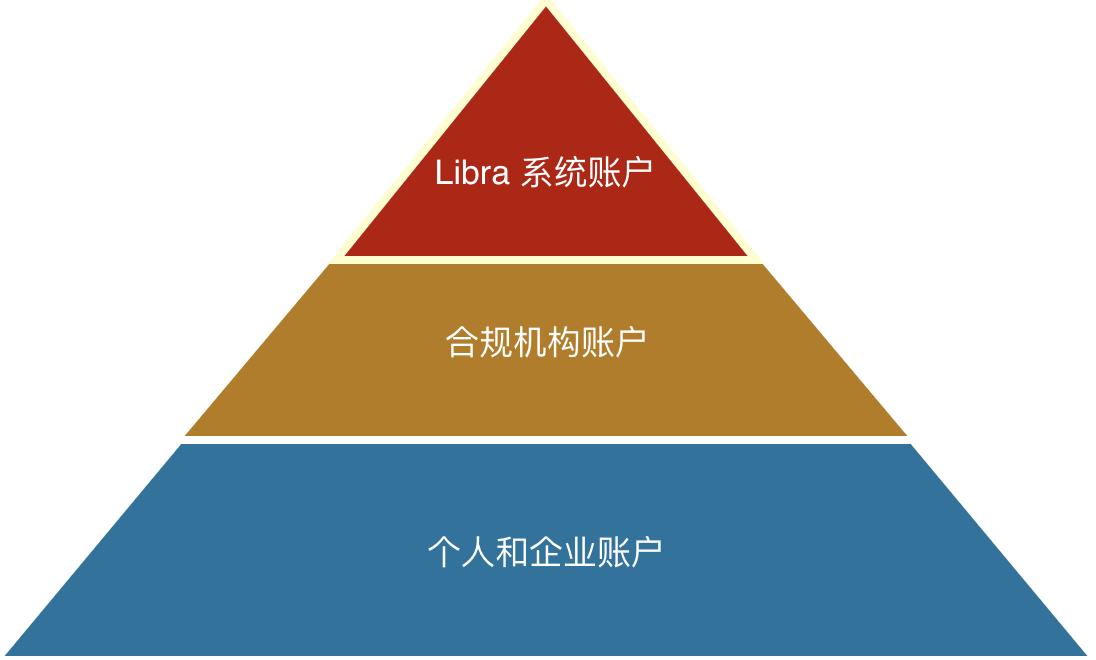
\includegraphics[width=10cm, keepaspectratio]{images/ledger_hierarchy.png}
    \caption{Libra 账户层次结构}
    \label{fig:hierarchy}
\end{figure}


%----------------------------------------------------------------------------------------
%	Section 8: 合规协议
%----------------------------------------------------------------------------------------
\section{合规验证协议}\label{sec:compliance}
根据PFMI\cite{pfmi}的附录四: "支付系统、证券结算系统、中央交易对手的设计纲要",典型的支付过程包括4个环节:
\begin{enumerate}
    \item 收单(Submission): 用户或者代理将支付指令提交给支付系统,指令一般包括发送方账户、接收方账户、额度、签名及其它相关的信息。
    \item 合规性审核(Validation): 接受指令后,支付系统审核支付双方的真实身份,根据所在司法辖区的要求,审核支付的合规性。
    \item 财务性审核(Conditionality): 合规性审核之后,还要通过财务性审核。主要是审核发送方是否有足够的余额,资产是否被冻结等等。
    \item 结算(Settlement): 最后,支付双方的账户完成结算,满足不可撤销性和最终性。
\end{enumerate}

在合规性审核(Validation)环节,金融机构要了解发送方的真实身份、接受方的真实身份,以及交易的背景数据,根据所属司法管辖区的要求审核该交易是否符合金融监管的要求。比如说根据反洗钱法的规定,要收集完整的、真实的、有效的交易背景数据,检查该交易是否涉嫌贩卖毒品、走私贸易、贪污贿赂等非法活动,是否隐瞒资产的来源和性质,试图将其合法化。

但是目前绝大多数分布式账本系统,缺少这种交易前置的手段保证交易的合规性。一般只能在交易之后,分析交易历史记录,追踪非法交易,手段被动而且低效。为了解决这个问题,这一章提出合规验证协议,通过此协议合规机构可以互相协作,验证每一笔交易的合规性。只有合规性检测通过之后,Libra 网络才会接受此交易。

本文只描述合规协议的基本框架和流程,并不是协议的详细规范说明。具体规范会在其它文档中另行说明。

根据第\ref{sec:arrangement}章“组织安排”,合规机构负责管理用户链下的KYC信息,以及审核用户的交易,所以合规审核的主体是合规机构。第\ref{sec:account_structure}章“账户数据结构”,提供了链上的账户与链下的身份管理系统集成方案,以及合规机构服务注册方案。这为合规审核协议提供了基础。

\subsection{典型交易场景}

为了叙述方便,我们先虚拟一个交易场景。不失一般性,假设有两家合规机构,分别为花旗银行(www.citi.com)与摩根大通银行(www.jpmorgan.com)。美国个人和企业可以向这两家合规机构提交真实身份数据,完成账户注册,并且委托他们执行合规审核。
他们的合规系统包括4部分::
\begin{enumerate}
    \item \textbf{KYC}子系统:      存储、管理个人与企业真实身份数据
    \item \textbf{Sanction}子系统: 存储、执行反洗钱(AML) 制裁规则,识别可能的洗钱活动。
    \item \textbf{Repository}子系统: 存储交易记录相关,提升交易透明度。
    \item \textbf{Compliance}子系统: 整合与封装 KYC、Sanction 与 Repository 内部子系统,对外提供合规服务 Rest API 接口,服务的地址保存在对应的 libra.toml 文件中。
\end{enumerate}

为了开展业务,首先他们需要向 Libra 协会实名注册,在 Libra 上建立知名账户,配置域名与 libra.toml文件。

\begin{figure}[h!]
    \centering
    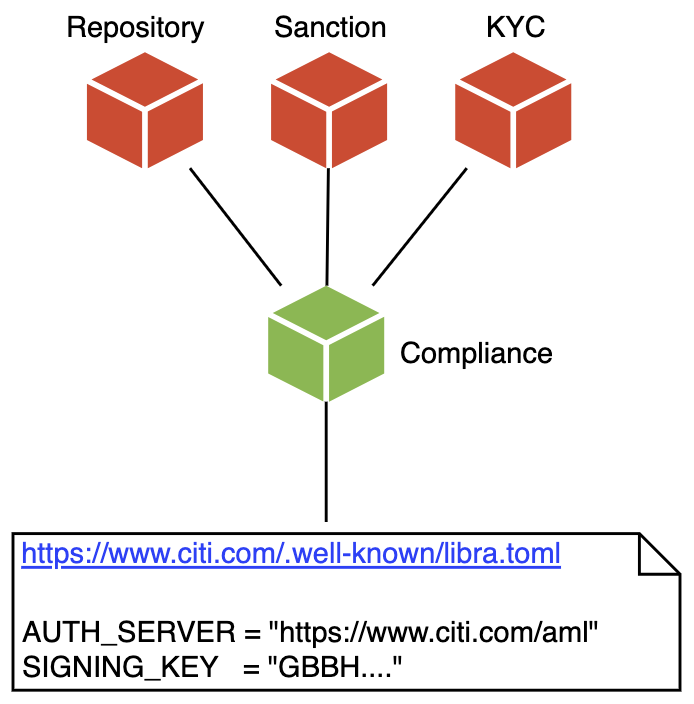
\includegraphics[width=8cm, keepaspectratio]{images/citi.png}
    \caption{花旗银行合规系统架构}
    \label{fig:citi}
\end{figure}


比如在花旗银行的 Libra 账户中,Domain 字段为 \url{www.citi.com},libra.toml 文件的URL为: \url{https://www.citi.com/.well-known/libra.toml}。
如图\ref{fig:citi}所示,其它机构可以通过此文件获取花旗银行的审核服务地址: \url{https://www.citi.com/aml}。

再假设有两个用户:Alice 和 Bob,他们分别向花旗银行与摩根大通银行实名注册,通过KYC审核流程之后,建立 libra 账户。比如,Alice 向花旗银行提交身份相关信息,建立 Libra 账户,账户中的 Validator 的字段是花旗银行的 Libra 账户地址。之后与 Alice 这个账户的所有交易需要花旗的审核通过才能结算。下图\ref{fig:accounts}显示这些账户的关键数据以及彼此之间的关联关系。

\begin{figure}[h!]
    \centering
    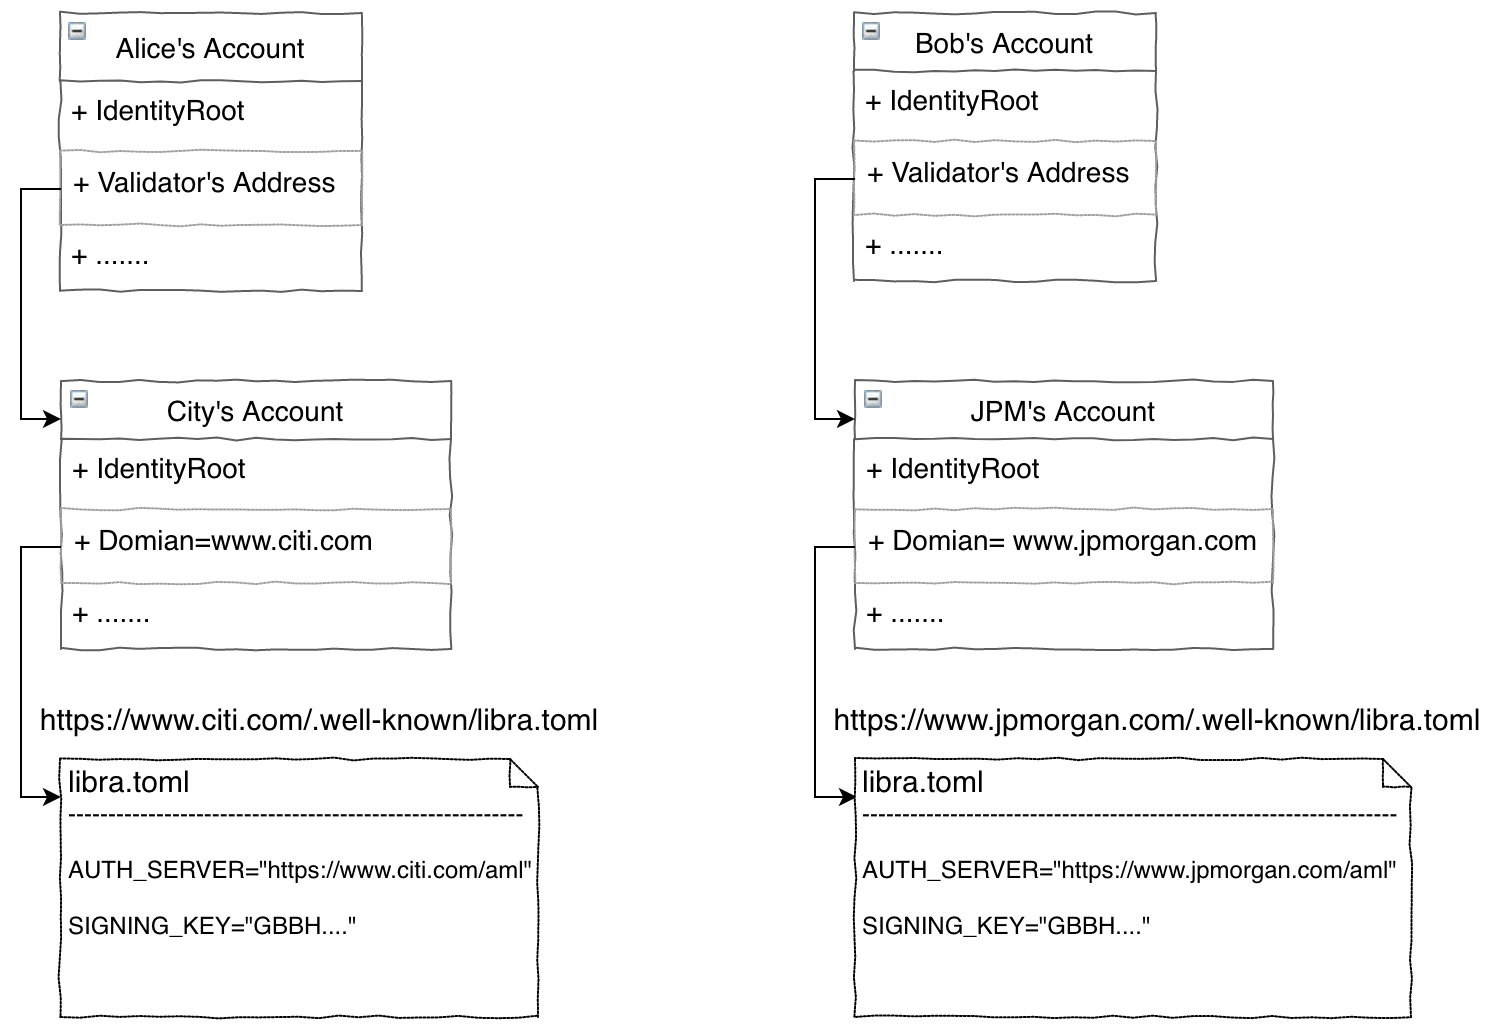
\includegraphics[width=10cm, keepaspectratio]{images/alice_bob.png}
    \caption{Alice、Bob、花旗、摩根大通的Libra账户}
    \label{fig:accounts}
\end{figure}

\subsection{合规审核服务}
每一家合规机构必须公布自己的交易审核服务。此服务根据所在司法辖区的规定,提供AML、CFT等合规审查,审查通过后对交易签名认证。从技术上讲,这是一个 Rest 风格的API服务,对应的服务 URL 地址和签名公钥公布在 libra.toml 文件里。 

%\subsubsection{审核服务消息}

在一个交易被广播到 Libra 网络之前,发送方的合规机构必须向接受方合规机构的审核服务发起请求。
这个请求是一个 HTTP POST 类型的请求,HTTP Header “Content-Type”的值必须为 “application/json”。
请求消息的正文部分是一个 JSON 格式的字符串,它的数据结构下图所示:

\begin{lstlisting}[caption={审核服务请求}, label={lst:auth_request}]
    {
        "data": {
            "sender": "<sender's address>",
            "need_info": "<whether need receiver's identity information>",
            "tx": "<hex string of transaction signed by sender>",
            "attachment": {
                "nonce": "<nounce>",
                "sender_info": {
                    "first_name": "<first_name>",
                    "middle_name": "<middle_name>",
                    "last_name": "<last_name>",
                    "address": "<address>",
                    "city": "<city>",
                    "province": "<province>",
                    "country": "<country in ISO 3166-1 alpha-2 format>",
                    "date_of_birth": "<date of birth in YYYY-MM-DD format>",
                    "company_name": "<company_name>"
                },
                "note": "<note>"
            }
        }
        "signature":"<the signature of data>"
    }
\end{lstlisting}

消息体中主要字段的含义如表\ref{tab:auth_req_field}所示:

\begin{table}[h]
    \caption{审核服务请求字段} 
    \label{tab:auth_req_field}
    \small % text size of table content
    \centering % center the table
    \begin{tabular}{lll} % alignment of each column data
        \toprule[\heavyrulewidth]\toprule[\heavyrulewidth]
        \textbf{名称} & \textbf{数据类型} & \textbf{描述} \\ 
        \midrule
        data.sender & string & 正在发起发送的客户的付款地址 \\
        data.need\_info & bool & 如果呼叫者需要收件人的AML信息才能发送付款 \\
        data.tx & string & base64编码格式交易信息 \\
        data.attachment & string & 附加的交易信息,便于合规机构的合规审查 \\
        signature & string & 合规机构的签名 \\
        \bottomrule[\heavyrulewidth] 
    \end{tabular}
\end{table}

响应的内容是如下结构的 JSON 格式字符串:

\begin{lstlisting}[caption={审核服务响应}, label={lst:auth_reply}]
    {
        "check_result": "<sanction check result for the transaction>",
        "info_result": "<whether share recipiant's identity information>",
        "recipiant_info":{
            "idendity_info": {
                "first_name": "<first_name>",
                "middle_name": "<middle_name>",
                "last_name": "<last_name>",
                "address": "<address>",
                "city": "<city>",
                "province": "<province>",
                "country": "<country in ISO 3166-1 alpha-2 format>",
                "date_of_birth": "<date of birth in YYYY-MM-DD format>",
                "company_name": "<company_name>"
                },
            "note": "<note>"
        }
    }
\end{lstlisting}

消息体中主要字段的含义如表\ref{tab:auth_reply_field}所示:

\begin{table}[h]
    \caption{审核服务响应字段} 
    \label{tab:auth_reply_field}
    \small % text size of table content
    \centering % center the table
    \begin{tabular}{lll} % alignment of each column data
        \toprule[\heavyrulewidth]\toprule[\heavyrulewidth]
        \textbf{名称} & \textbf{数据类型} & \textbf{描述} \\ 
        \midrule
        check\_result & ok,denied & 接收方合规机构是否愿意接受此交易 \\
        info\_result & ok,denied & 接收方合规机构是否愿意分享反洗钱信息 \\
        recipiant\_info & string &  接收方 AML信息 \\
        \bottomrule[\heavyrulewidth] 
    \end{tabular}
\end{table}

接收方合规机构的返回的HTTP状态代码可以是:
\begin{table}[h]
    \caption{审核服务响应HTTP状态代码} 
    \label{tab:auth_http_status}
    \small % text size of table content
    \centering % center the table
    \begin{tabular}{lll} % alignment of each column data
        \toprule[\heavyrulewidth]\toprule[\heavyrulewidth]
        \textbf{状态码} & \textbf{状态} & \textbf{描述} \\ 
        \midrule
        200 & OK & 如果 info\_result 和 check\_status 的值为 OK \\
        202 & Accepted &  如果 info\_result的值为 pending, check\_status的值为 OK,\\
        400 & Bad Request &  如果发件人发送的数据无效。\\
        403 & Forbidden &  如果任何 info\_result 或者 check\_status 的值为 denied\\
        500 & Internal Server Error &  服务器端有内部错误 \\
        \bottomrule[\heavyrulewidth] 
    \end{tabular}
\end{table}

\subsection{合规流程}

对于一笔交易,交易双方所注册的合规机构可能不是一家,任何一家合规机构只有一方的相关身份信息,两家合规机构需要彼此通信才能获得完整的KYC数据、完成合规检查。在某些司法管辖区,合规机构能够信任另一方合规机构的的审核结果;而在另一些司法管辖区,每家合规机构必须收集完整的KYC数据独立进行制裁检查,而且需要双方都审核通过。本文以后者双方公审为例,介绍合规流程。

如下图\ref{fig:compliance}所示,Alice 向 Bob 发起一个支付请求。和其它分布式账本不同的是,这个交易请求不是直接广播到 Libra 网络上,而是先要提交给花旗做预处理,如果花旗和摩根两家合规机构都审核通过,然后再广播到 Libra 网络上确认记账。具体的过程包含以下十个步骤:

\begin{figure}[h!]
    \centering
    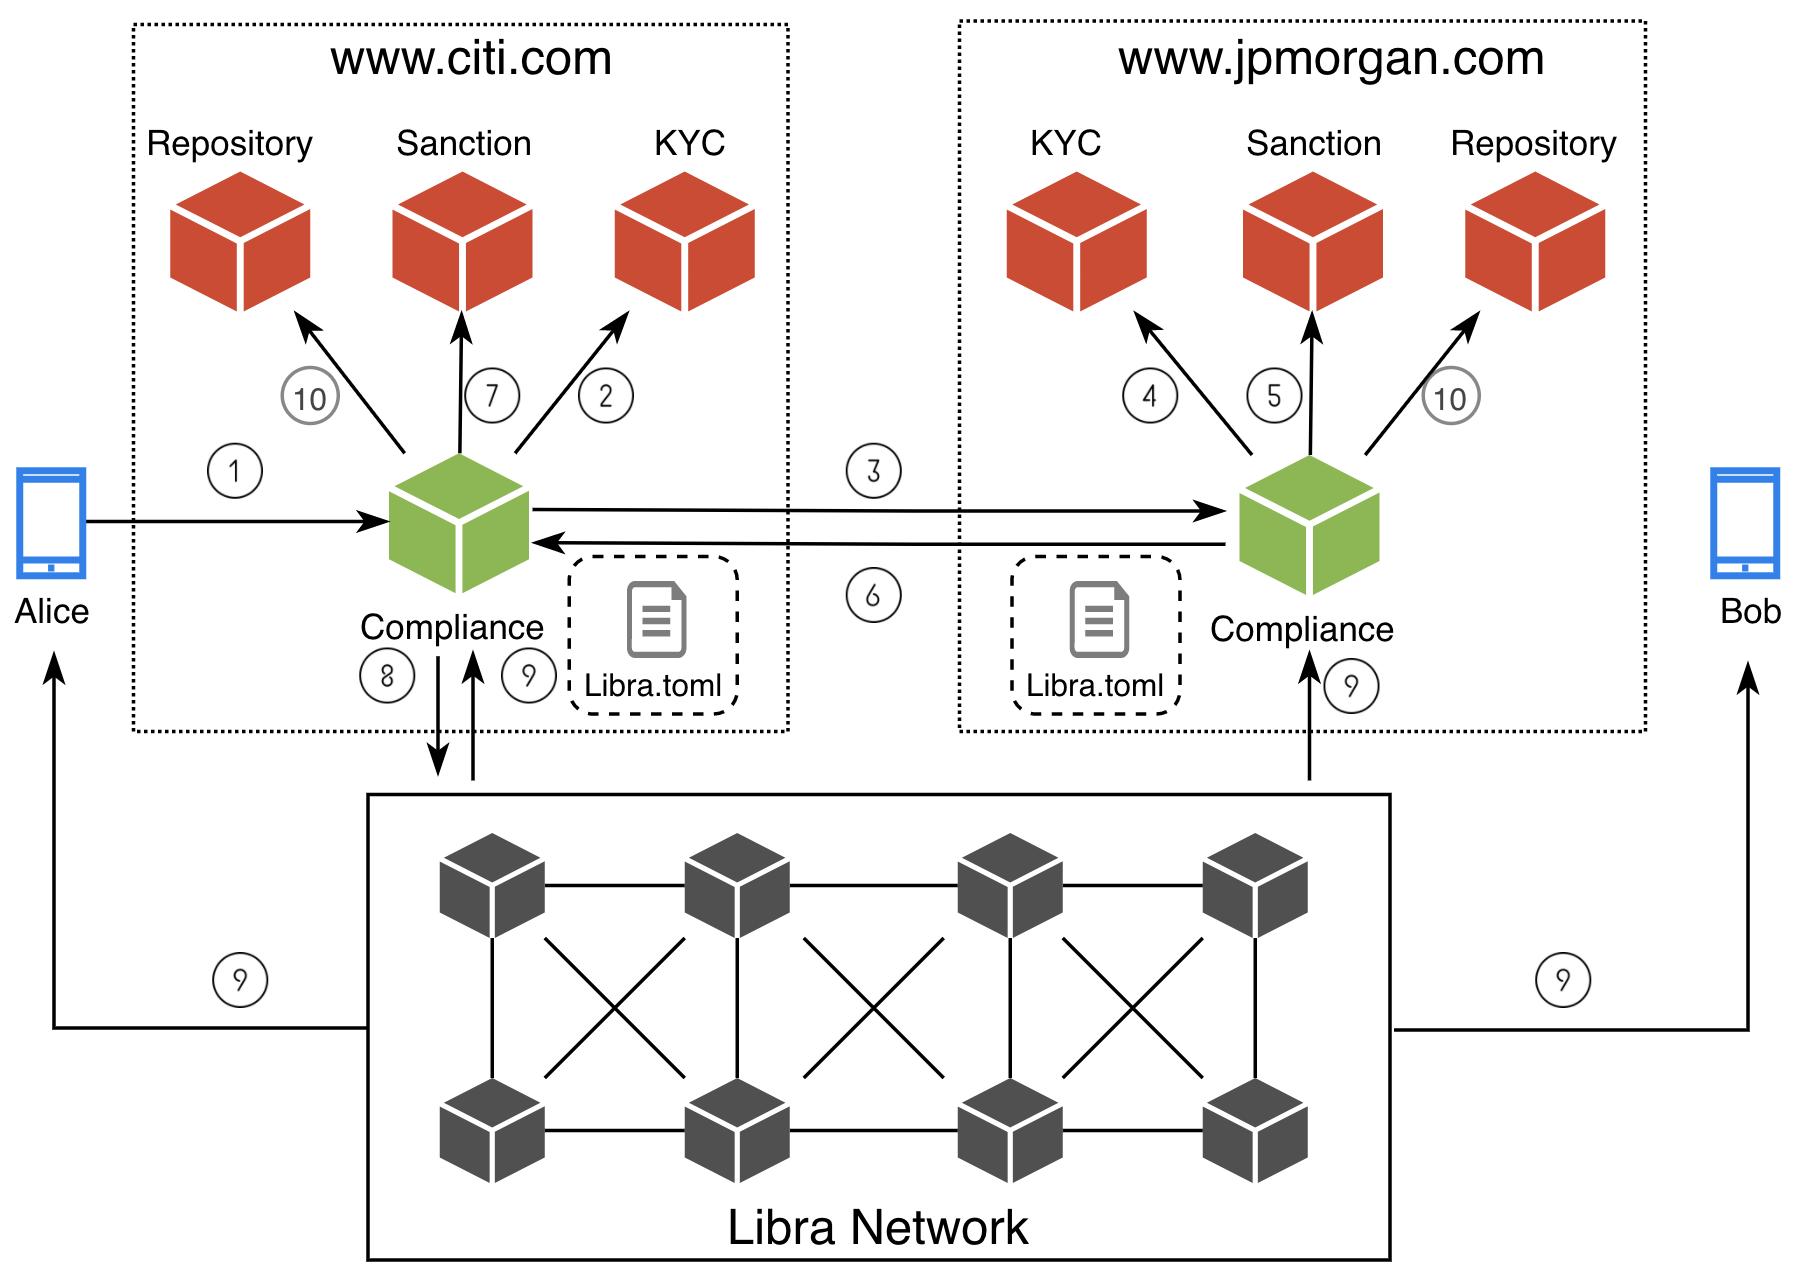
\includegraphics[width=12cm, keepaspectratio]{images/compliance.png}
    \caption{合规审核流程}
    \label{fig:compliance}
\end{figure}
\begin{enumerate}
    \item Alice 获取 Bob 的身份账户与资产账户,构建一个交易请求并且签名。Alice 通过花旗银行的 libra.toml 文件获取合规服务的URL,将签名后的交易提交给花旗银行的合规服务处理。
    
    \begin{lstlisting}[caption={Alice 请求花旗银行审核交易}, label={lst:alice_request}]
    POST https://www.citi.com/aml/newTx      HTTP/1.1
    Content-Type:   application/json
    {
        "data": {
            "sender": "<Alice's identity account>",
            "recipiant": "<Bob's identity account>",
            "tx": "<hex string of transaction signed with Alice's asset account>",
            "note": "<note about the transaction>"
        }
        "signature":"<Alice's signature of data field>"
    }
    \end{lstlisting}

    \item 花旗银行的合规服务收到 Alice 的请求之后,先查询本地的 KYC 服务,确认 Alice 的身份信息。

    \item 花旗银行解析 Bob 的身份账户数据,判定接收方的合规机构是摩根银行。然后找到摩根银行的合规服务URL。将 Alice 的交易与 KYC 数据打包,请求摩根银行根据 Alice 和 Bob 的KYC数据审核该交易是否受AML制裁限制,同时也请求返回 Bob 的KYC数据。

    \begin{lstlisting}[caption={花旗银行请求摩根银行审核交易}, label={lst:citi_request}]
    POST https://www.jpmorgan.com/aml/sanctionCheck      HTTP/1.1
    Content-Type:   application/json
    {
        "data": {
            "sender": "<Alice's account>",
            "need_recipiant_info": "Yes",
            "tx": "<hex string of transaction signed with Alice's asset account>",
            "attachment": {
                "nonce": "<nounce>",
                "sender_info": {
                    "first_name": "<Alice's first_name>",
                    "middle_name": "<Alice's middle_name>",
                    "last_name": "<Alice's last_name>",
                    "address": "<Alice's address>",
                    "city": "<Alice's city>",
                    "province": "<Alice's province>",
                    "country": "<Alice's nationality>",
                    "date_of_birth": "<Alice's birthday>",
                    "company_name": "<Alice's company name>"
                },
                "note": "<note about the transaction>"
            }
        }
        "signature":"<the signature of data by Citi Bank>"
    }
    \end{lstlisting}

    \item 摩根银行的合规服务收到花旗的请求之后,先查询本地的 KYC 服务,确认 Bob 的身份信息。

    \item 摩根银行调用内部的 Sanction 子系统,审核此交易是否涉嫌洗钱。

    \item 如果通过AML制裁检查,摩根将审核的结果返回给花旗银行,并且将 Bob 的身份信息一并返回。

    \begin{lstlisting}[caption={摩根银行向花旗银行返回审核结果}, label={lst:jpm_reply}]
    HTTP/1.1 200 OK
    Content-Type:   application/json
    {
        "check_result": "ok",
        "info_result": "yes",
        "recipiant_info":{
            "first_name": "<Bob's first_name>",
            "middle_name": "<Bob's middle_name>",
            "last_name": "<Bob's last_name>",
            "address": "<Bob's address>",
            "city": "<Bob's city>",
            "province": "<Bob's province>",
            "country": "<Bob's nationality>",
            "date_of_birth": "<Bob's birthday>",
            "company_name": "<Bob's company name>"
        }
        "signature":"<the signature of recipiant_info by JPM Bank>"
    }
    \end{lstlisting}

    \item 花旗银行获得 Bob 的身份信息后,与 Alice 的身份合并,根据本地的 Sanction 规则,重新审核此交易是否涉嫌洗钱。

    \item 如果花旗银行的AML制裁检查也通过,那么花旗银行对于此交易签名,广播到 Libra 网络上。所以此交易不仅仅包含 Alice 的签名,也包含花旗银行的签名。

    \item Libra 的矿工们收到未确认的交易,检查是否满足确认条件。验证的条件至少包括下列几项:
        \begin{itemize}
            \item   检查 花旗银行的签名,验证交易是否已经审核通过。
            \item   检查 Alice 的签名,验证其是否为发送账户的拥有者
            \item   检查 Alice 的资产账户余额是否充足等其它必要条件
        \end{itemize}
        以上条件都通过之后,所有矿工达成共识将此交易写入 Libra 账本。之后的全网同步过程中,Alice、Bob、花旗和摩根银行都会收到交易确认消息。

    \item 花旗和摩根银行将确认后的交易数据写入本地的 Trade Repository 归档,以备之后的审查。归档记录里面包含以下数据
        \begin{itemize}
            \item   发送方的相关信息: Alice 的身份信息、转出资产账户。
            \item   发送方合规机构的签名: 花旗银行的签名
            \item   接受方的相关信息: Bob 的身份信息、转入资产账户。
            \item   接受方合规机构的签名: 摩根银行的签名
            \item   交易的相关信息: 交易时间,额度等
        \end{itemize}
        这些归档数据可以向有关管理部门提供详尽、准确的历史数据,提高市场透明度,并支持相关公共政策目标。
\end{enumerate}



%----------------------------------------------------------------------------------------
%	Section 9: 智能合约
%----------------------------------------------------------------------------------------
%\section{合规验证协议}\label{sec:compliance}
根据PFMI\cite{pfmi}的附录四: "支付系统、证券结算系统、中央交易对手的设计纲要",典型的支付过程包括4个环节:
\begin{enumerate}
    \item 收单(Submission): 用户或者代理将支付指令提交给支付系统,指令一般包括发送方账户、接收方账户、额度、签名及其它相关的信息。
    \item 合规性审核(Validation): 接受指令后,支付系统审核支付双方的真实身份,根据所在司法辖区的要求,审核支付的合规性。
    \item 财务性审核(Conditionality): 合规性审核之后,还要通过财务性审核。主要是审核发送方是否有足够的余额,资产是否被冻结等等。
    \item 结算(Settlement): 最后,支付双方的账户完成结算,满足不可撤销性和最终性。
\end{enumerate}

在合规性审核(Validation)环节,金融机构要了解发送方的真实身份、接受方的真实身份,以及交易的背景数据,根据所属司法管辖区的要求审核该交易是否符合金融监管的要求。比如说根据反洗钱法的规定,要收集完整的、真实的、有效的交易背景数据,检查该交易是否涉嫌贩卖毒品、走私贸易、贪污贿赂等非法活动,是否隐瞒资产的来源和性质,试图将其合法化。

但是目前绝大多数分布式账本系统,缺少这种交易前置的手段保证交易的合规性。一般只能在交易之后,分析交易历史记录,追踪非法交易,手段被动而且低效。为了解决这个问题,这一章提出合规验证协议,通过此协议合规机构可以互相协作,验证每一笔交易的合规性。只有合规性检测通过之后,Libra 网络才会接受此交易。

本文只描述合规协议的基本框架和流程,并不是协议的详细规范说明。具体规范会在其它文档中另行说明。

根据第\ref{sec:arrangement}章“组织安排”,合规机构负责管理用户链下的KYC信息,以及审核用户的交易,所以合规审核的主体是合规机构。第\ref{sec:account_structure}章“账户数据结构”,提供了链上的账户与链下的身份管理系统集成方案,以及合规机构服务注册方案。这为合规审核协议提供了基础。

\subsection{典型交易场景}

为了叙述方便,我们先虚拟一个交易场景。不失一般性,假设有两家合规机构,分别为花旗银行(www.citi.com)与摩根大通银行(www.jpmorgan.com)。美国个人和企业可以向这两家合规机构提交真实身份数据,完成账户注册,并且委托他们执行合规审核。
他们的合规系统包括4部分::
\begin{enumerate}
    \item \textbf{KYC}子系统:      存储、管理个人与企业真实身份数据
    \item \textbf{Sanction}子系统: 存储、执行反洗钱(AML) 制裁规则,识别可能的洗钱活动。
    \item \textbf{Repository}子系统: 存储交易记录相关,提升交易透明度。
    \item \textbf{Compliance}子系统: 整合与封装 KYC、Sanction 与 Repository 内部子系统,对外提供合规服务 Rest API 接口,服务的地址保存在对应的 libra.toml 文件中。
\end{enumerate}

为了开展业务,首先他们需要向 Libra 协会实名注册,在 Libra 上建立知名账户,配置域名与 libra.toml文件。

\begin{figure}[h!]
    \centering
    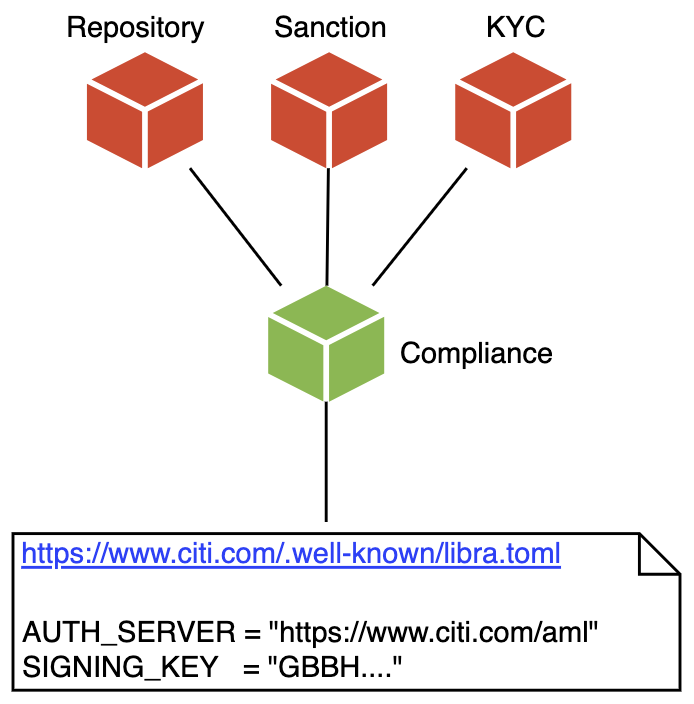
\includegraphics[width=8cm, keepaspectratio]{images/citi.png}
    \caption{花旗银行合规系统架构}
    \label{fig:citi}
\end{figure}


比如在花旗银行的 Libra 账户中,Domain 字段为 \url{www.citi.com},libra.toml 文件的URL为: \url{https://www.citi.com/.well-known/libra.toml}。
如图\ref{fig:citi}所示,其它机构可以通过此文件获取花旗银行的审核服务地址: \url{https://www.citi.com/aml}。

再假设有两个用户:Alice 和 Bob,他们分别向花旗银行与摩根大通银行实名注册,通过KYC审核流程之后,建立 libra 账户。比如,Alice 向花旗银行提交身份相关信息,建立 Libra 账户,账户中的 Validator 的字段是花旗银行的 Libra 账户地址。之后与 Alice 这个账户的所有交易需要花旗的审核通过才能结算。下图\ref{fig:accounts}显示这些账户的关键数据以及彼此之间的关联关系。

\begin{figure}[h!]
    \centering
    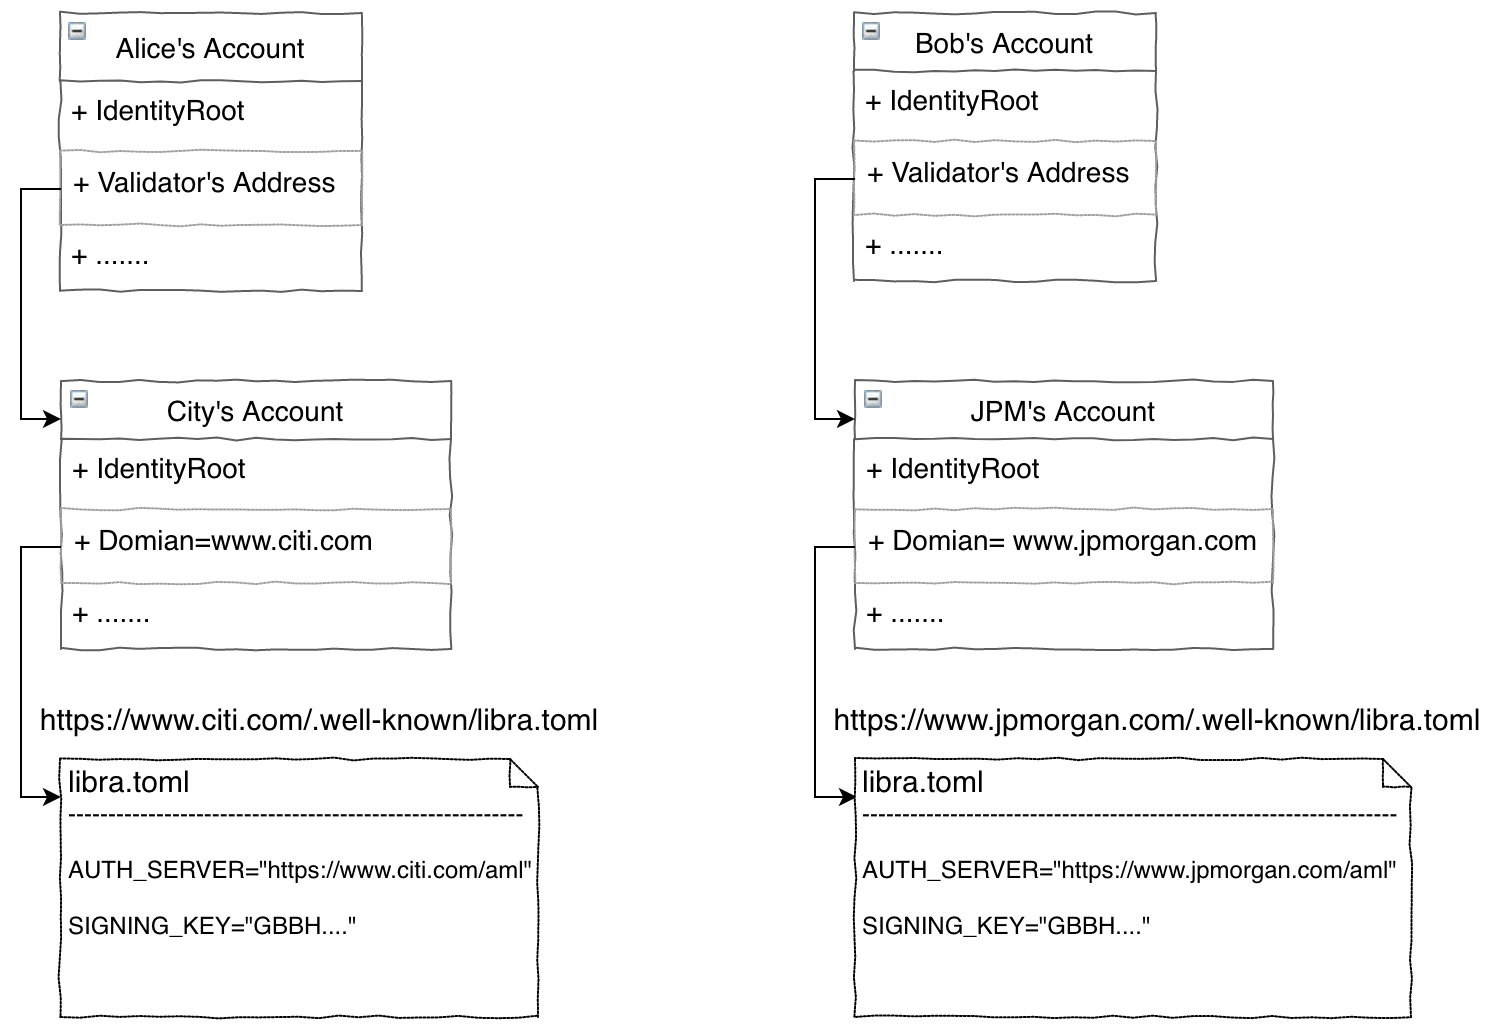
\includegraphics[width=10cm, keepaspectratio]{images/alice_bob.png}
    \caption{Alice、Bob、花旗、摩根大通的Libra账户}
    \label{fig:accounts}
\end{figure}

\subsection{合规审核服务}
每一家合规机构必须公布自己的交易审核服务。此服务根据所在司法辖区的规定,提供AML、CFT等合规审查,审查通过后对交易签名认证。从技术上讲,这是一个 Rest 风格的API服务,对应的服务 URL 地址和签名公钥公布在 libra.toml 文件里。 

%\subsubsection{审核服务消息}

在一个交易被广播到 Libra 网络之前,发送方的合规机构必须向接受方合规机构的审核服务发起请求。
这个请求是一个 HTTP POST 类型的请求,HTTP Header “Content-Type”的值必须为 “application/json”。
请求消息的正文部分是一个 JSON 格式的字符串,它的数据结构下图所示:

\begin{lstlisting}[caption={审核服务请求}, label={lst:auth_request}]
    {
        "data": {
            "sender": "<sender's address>",
            "need_info": "<whether need receiver's identity information>",
            "tx": "<hex string of transaction signed by sender>",
            "attachment": {
                "nonce": "<nounce>",
                "sender_info": {
                    "first_name": "<first_name>",
                    "middle_name": "<middle_name>",
                    "last_name": "<last_name>",
                    "address": "<address>",
                    "city": "<city>",
                    "province": "<province>",
                    "country": "<country in ISO 3166-1 alpha-2 format>",
                    "date_of_birth": "<date of birth in YYYY-MM-DD format>",
                    "company_name": "<company_name>"
                },
                "note": "<note>"
            }
        }
        "signature":"<the signature of data>"
    }
\end{lstlisting}

消息体中主要字段的含义如表\ref{tab:auth_req_field}所示:

\begin{table}[h]
    \caption{审核服务请求字段} 
    \label{tab:auth_req_field}
    \small % text size of table content
    \centering % center the table
    \begin{tabular}{lll} % alignment of each column data
        \toprule[\heavyrulewidth]\toprule[\heavyrulewidth]
        \textbf{名称} & \textbf{数据类型} & \textbf{描述} \\ 
        \midrule
        data.sender & string & 正在发起发送的客户的付款地址 \\
        data.need\_info & bool & 如果呼叫者需要收件人的AML信息才能发送付款 \\
        data.tx & string & base64编码格式交易信息 \\
        data.attachment & string & 附加的交易信息,便于合规机构的合规审查 \\
        signature & string & 合规机构的签名 \\
        \bottomrule[\heavyrulewidth] 
    \end{tabular}
\end{table}

响应的内容是如下结构的 JSON 格式字符串:

\begin{lstlisting}[caption={审核服务响应}, label={lst:auth_reply}]
    {
        "check_result": "<sanction check result for the transaction>",
        "info_result": "<whether share recipiant's identity information>",
        "recipiant_info":{
            "idendity_info": {
                "first_name": "<first_name>",
                "middle_name": "<middle_name>",
                "last_name": "<last_name>",
                "address": "<address>",
                "city": "<city>",
                "province": "<province>",
                "country": "<country in ISO 3166-1 alpha-2 format>",
                "date_of_birth": "<date of birth in YYYY-MM-DD format>",
                "company_name": "<company_name>"
                },
            "note": "<note>"
        }
    }
\end{lstlisting}

消息体中主要字段的含义如表\ref{tab:auth_reply_field}所示:

\begin{table}[h]
    \caption{审核服务响应字段} 
    \label{tab:auth_reply_field}
    \small % text size of table content
    \centering % center the table
    \begin{tabular}{lll} % alignment of each column data
        \toprule[\heavyrulewidth]\toprule[\heavyrulewidth]
        \textbf{名称} & \textbf{数据类型} & \textbf{描述} \\ 
        \midrule
        check\_result & ok,denied & 接收方合规机构是否愿意接受此交易 \\
        info\_result & ok,denied & 接收方合规机构是否愿意分享反洗钱信息 \\
        recipiant\_info & string &  接收方 AML信息 \\
        \bottomrule[\heavyrulewidth] 
    \end{tabular}
\end{table}

接收方合规机构的返回的HTTP状态代码可以是:
\begin{table}[h]
    \caption{审核服务响应HTTP状态代码} 
    \label{tab:auth_http_status}
    \small % text size of table content
    \centering % center the table
    \begin{tabular}{lll} % alignment of each column data
        \toprule[\heavyrulewidth]\toprule[\heavyrulewidth]
        \textbf{状态码} & \textbf{状态} & \textbf{描述} \\ 
        \midrule
        200 & OK & 如果 info\_result 和 check\_status 的值为 OK \\
        202 & Accepted &  如果 info\_result的值为 pending, check\_status的值为 OK,\\
        400 & Bad Request &  如果发件人发送的数据无效。\\
        403 & Forbidden &  如果任何 info\_result 或者 check\_status 的值为 denied\\
        500 & Internal Server Error &  服务器端有内部错误 \\
        \bottomrule[\heavyrulewidth] 
    \end{tabular}
\end{table}

\subsection{合规流程}

对于一笔交易,交易双方所注册的合规机构可能不是一家,任何一家合规机构只有一方的相关身份信息,两家合规机构需要彼此通信才能获得完整的KYC数据、完成合规检查。在某些司法管辖区,合规机构能够信任另一方合规机构的的审核结果;而在另一些司法管辖区,每家合规机构必须收集完整的KYC数据独立进行制裁检查,而且需要双方都审核通过。本文以后者双方公审为例,介绍合规流程。

如下图\ref{fig:compliance}所示,Alice 向 Bob 发起一个支付请求。和其它分布式账本不同的是,这个交易请求不是直接广播到 Libra 网络上,而是先要提交给花旗做预处理,如果花旗和摩根两家合规机构都审核通过,然后再广播到 Libra 网络上确认记账。具体的过程包含以下十个步骤:

\begin{figure}[h!]
    \centering
    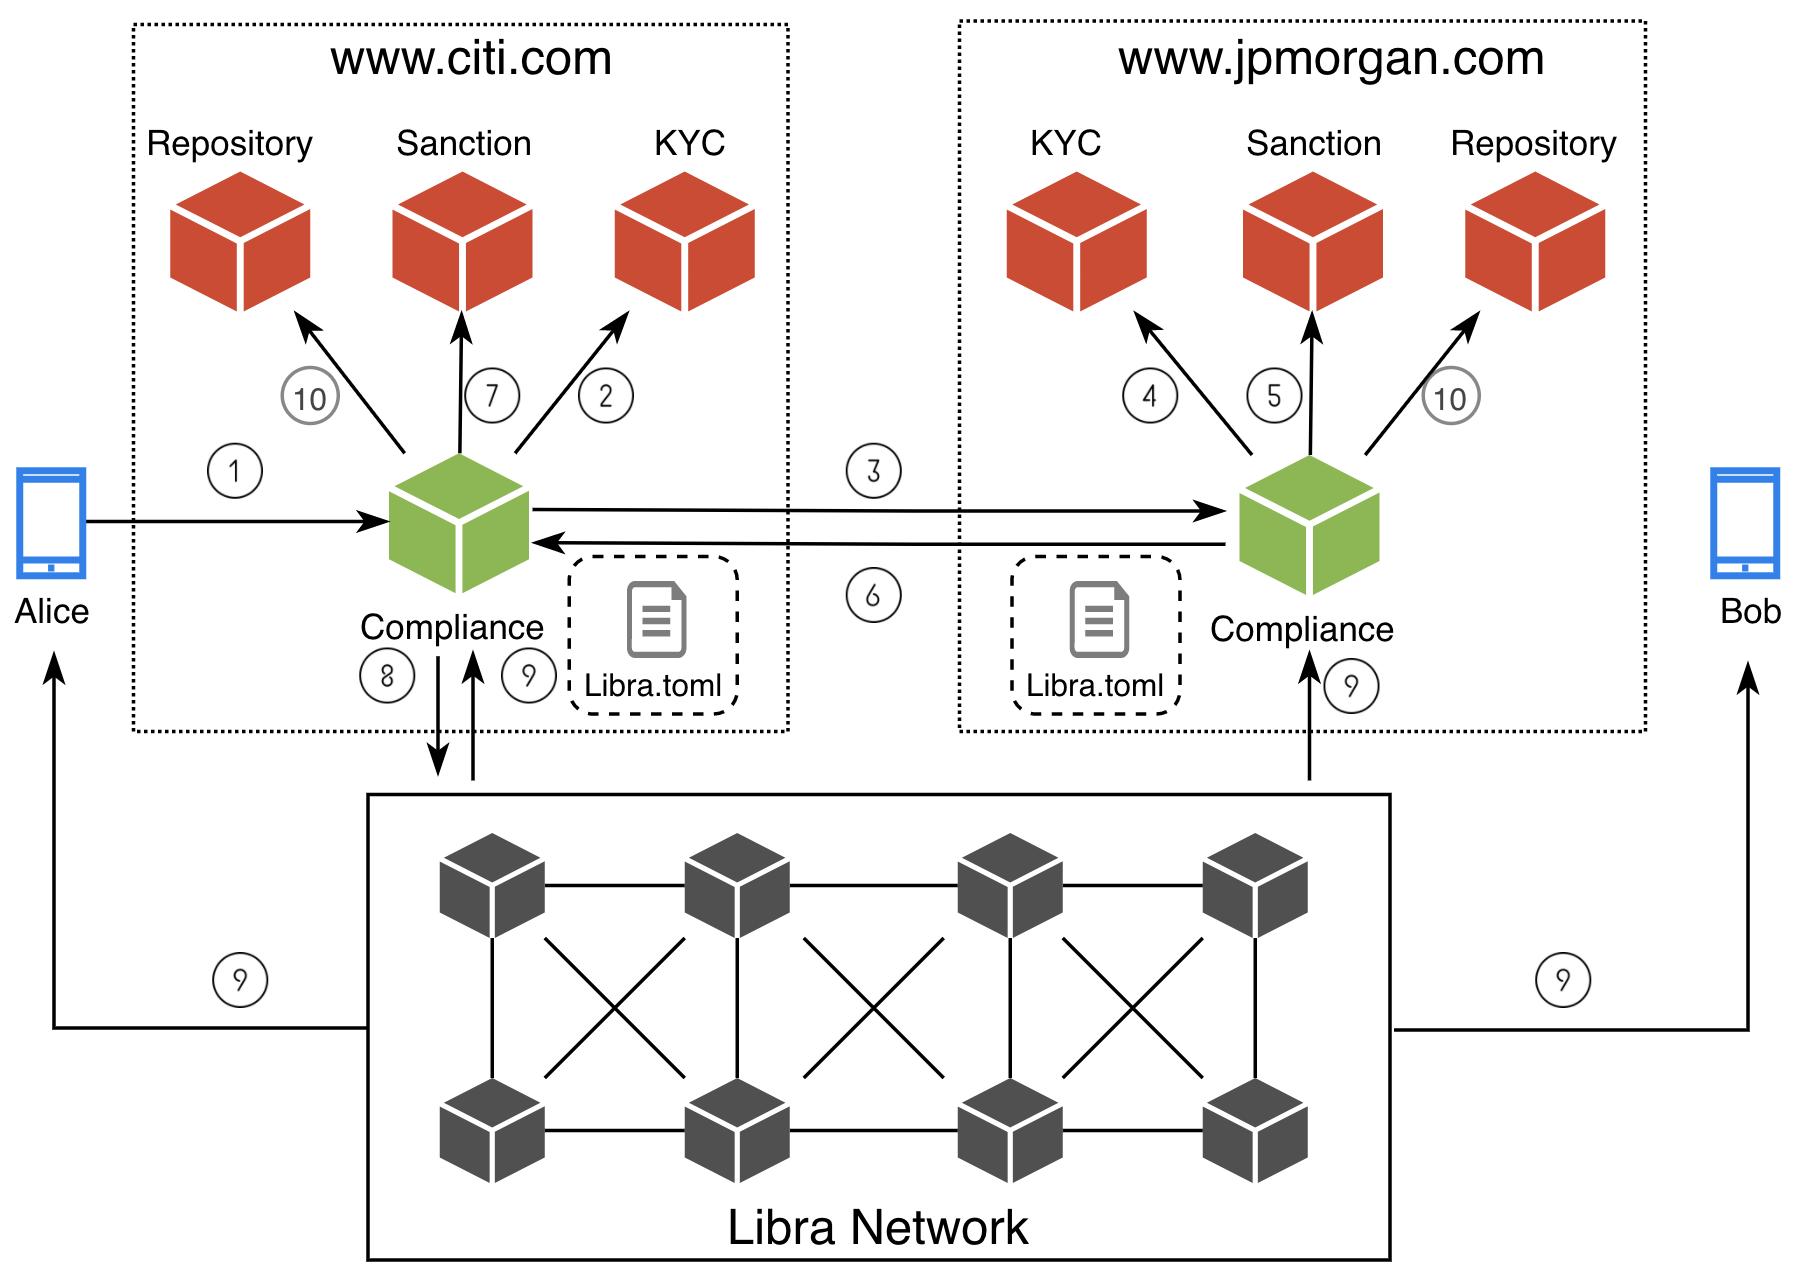
\includegraphics[width=12cm, keepaspectratio]{images/compliance.png}
    \caption{合规审核流程}
    \label{fig:compliance}
\end{figure}
\begin{enumerate}
    \item Alice 获取 Bob 的身份账户与资产账户,构建一个交易请求并且签名。Alice 通过花旗银行的 libra.toml 文件获取合规服务的URL,将签名后的交易提交给花旗银行的合规服务处理。
    
    \begin{lstlisting}[caption={Alice 请求花旗银行审核交易}, label={lst:alice_request}]
    POST https://www.citi.com/aml/newTx      HTTP/1.1
    Content-Type:   application/json
    {
        "data": {
            "sender": "<Alice's identity account>",
            "recipiant": "<Bob's identity account>",
            "tx": "<hex string of transaction signed with Alice's asset account>",
            "note": "<note about the transaction>"
        }
        "signature":"<Alice's signature of data field>"
    }
    \end{lstlisting}

    \item 花旗银行的合规服务收到 Alice 的请求之后,先查询本地的 KYC 服务,确认 Alice 的身份信息。

    \item 花旗银行解析 Bob 的身份账户数据,判定接收方的合规机构是摩根银行。然后找到摩根银行的合规服务URL。将 Alice 的交易与 KYC 数据打包,请求摩根银行根据 Alice 和 Bob 的KYC数据审核该交易是否受AML制裁限制,同时也请求返回 Bob 的KYC数据。

    \begin{lstlisting}[caption={花旗银行请求摩根银行审核交易}, label={lst:citi_request}]
    POST https://www.jpmorgan.com/aml/sanctionCheck      HTTP/1.1
    Content-Type:   application/json
    {
        "data": {
            "sender": "<Alice's account>",
            "need_recipiant_info": "Yes",
            "tx": "<hex string of transaction signed with Alice's asset account>",
            "attachment": {
                "nonce": "<nounce>",
                "sender_info": {
                    "first_name": "<Alice's first_name>",
                    "middle_name": "<Alice's middle_name>",
                    "last_name": "<Alice's last_name>",
                    "address": "<Alice's address>",
                    "city": "<Alice's city>",
                    "province": "<Alice's province>",
                    "country": "<Alice's nationality>",
                    "date_of_birth": "<Alice's birthday>",
                    "company_name": "<Alice's company name>"
                },
                "note": "<note about the transaction>"
            }
        }
        "signature":"<the signature of data by Citi Bank>"
    }
    \end{lstlisting}

    \item 摩根银行的合规服务收到花旗的请求之后,先查询本地的 KYC 服务,确认 Bob 的身份信息。

    \item 摩根银行调用内部的 Sanction 子系统,审核此交易是否涉嫌洗钱。

    \item 如果通过AML制裁检查,摩根将审核的结果返回给花旗银行,并且将 Bob 的身份信息一并返回。

    \begin{lstlisting}[caption={摩根银行向花旗银行返回审核结果}, label={lst:jpm_reply}]
    HTTP/1.1 200 OK
    Content-Type:   application/json
    {
        "check_result": "ok",
        "info_result": "yes",
        "recipiant_info":{
            "first_name": "<Bob's first_name>",
            "middle_name": "<Bob's middle_name>",
            "last_name": "<Bob's last_name>",
            "address": "<Bob's address>",
            "city": "<Bob's city>",
            "province": "<Bob's province>",
            "country": "<Bob's nationality>",
            "date_of_birth": "<Bob's birthday>",
            "company_name": "<Bob's company name>"
        }
        "signature":"<the signature of recipiant_info by JPM Bank>"
    }
    \end{lstlisting}

    \item 花旗银行获得 Bob 的身份信息后,与 Alice 的身份合并,根据本地的 Sanction 规则,重新审核此交易是否涉嫌洗钱。

    \item 如果花旗银行的AML制裁检查也通过,那么花旗银行对于此交易签名,广播到 Libra 网络上。所以此交易不仅仅包含 Alice 的签名,也包含花旗银行的签名。

    \item Libra 的矿工们收到未确认的交易,检查是否满足确认条件。验证的条件至少包括下列几项:
        \begin{itemize}
            \item   检查 花旗银行的签名,验证交易是否已经审核通过。
            \item   检查 Alice 的签名,验证其是否为发送账户的拥有者
            \item   检查 Alice 的资产账户余额是否充足等其它必要条件
        \end{itemize}
        以上条件都通过之后,所有矿工达成共识将此交易写入 Libra 账本。之后的全网同步过程中,Alice、Bob、花旗和摩根银行都会收到交易确认消息。

    \item 花旗和摩根银行将确认后的交易数据写入本地的 Trade Repository 归档,以备之后的审查。归档记录里面包含以下数据
        \begin{itemize}
            \item   发送方的相关信息: Alice 的身份信息、转出资产账户。
            \item   发送方合规机构的签名: 花旗银行的签名
            \item   接受方的相关信息: Bob 的身份信息、转入资产账户。
            \item   接受方合规机构的签名: 摩根银行的签名
            \item   交易的相关信息: 交易时间,额度等
        \end{itemize}
        这些归档数据可以向有关管理部门提供详尽、准确的历史数据,提高市场透明度,并支持相关公共政策目标。
\end{enumerate}



%----------------------------------------------------------------------------------------
%	Section 10: 结论
%----------------------------------------------------------------------------------------
\section{结语}

分布式账本技术的发展为构建新一代金融基础设施带来了希望,但是长期以来,监管与合规的需求并没有得到业界普遍的重视,也缺少充分的研究和可行的解决方案。本文不仅仅从理论上分析了监管与合规的挑战,而且总结了前人工作的经验教训。在此基础上提出了一套可行的合规解决方案,填补了业界的空白。

我们坚信,重新构建金融行业的基础设施是一个划时代的机会。要实现这样的愿景,绝非一己之力可以完成,需要精心设计的方案、长久的艰辛努力、以及多方紧密的协作。希望本文提出的监管与合规相关技术方案,能够得到业界的广泛共识,促进分布式账本技术加速应用于金融领域,创造更完善、更实惠的开放式金融服务。


%----------------------------------------------------------------------------------------
%	Appendix A: 源码技术详解
%----------------------------------------------------------------------------------------
%\pagebreak
%\input{A_Source_Code.tex}



%----------------------------------------------------------------------------------------
%	BIBLIOGRAPHY
%----------------------------------------------------------------------------------------
%\pagebreak

%----------------------------------------------------------------------------------------
%	REFERENCE LIST
%----------------------------------------------------------------------------------------
\newpage

%----------------------------------------------------------------------------------------
%	BIBLIOGRAPHY
%----------------------------------------------------------------------------------------


\bibliographystyle{unsrt}
%\bibliography{sample.bib}

\begin{thebibliography}{99} % Bibliography - this is intentionally simple in this template

    \bibitem{btc_wp} Satoshi Nakamoto,
    \newblock \textit{Bitcoin: A peer-to-peer electronic cash system.}
    \newblock \textbf{2008,}
    \newblock \url{https://bitcoin.org/bitcoin.pdf}.
        
    \bibitem{eth_wp} Vitalik Buterin,
    \newblock \textit{Ethereum: a next generation smart contract and decentralized application platform.}
    \newblock \textbf{2013,}
    \newblock \url{https://github.com/ethereum/wiki/wiki/White-Paper}.
    
    \bibitem{jp_report} 日本国家警察局,
    \newblock \textit{Cases of money laundering linked to cryptocurrency in Japan up tenfold in 2018,}
    \newblock \url{https://www.japantimes.co.jp/news/2019/02/28/national/crime-legal/cases-money-laundering-linked-cryptocurrency-japan-tenfold-2018/#.XS6LyZP7QlL}.
    
    \bibitem{pfmi} 世界清算银行(BIS) 和国际证监会组织(IOSCO),
    \newblock \textbf{2012,}
    \newblock \textit{Principles for financial market infrastructures,}
    \newblock \url{https://www.bis.org/publ/cpss101a.pdf}.

    \bibitem{bis_dlt} 世界清算银行(BIS) ,
    \newblock \textit{Distributed ledger technology in payment, clearing and settlement - an analytical framework,}
    \newblock \textbf{2017,}
    \newblock \url{https://www.bis.org/cpmi/publ/d157.htm}.
    
    \bibitem{fr} 美联储 ,
    \newblock \textit{Distributed ledger technology in payments, clearing, and settlement,}
    \newblock \textbf{2016,}
    \newblock \url{https://www.federalreserve.gov/econresdata/feds/2016/files/2016095pap.pdf}.

    \bibitem{dtcc} 美国存管信托与清算公司(DTCC),
    \newblock \textit{Embracing Disruption: Tapping the Potential of Distributed Ledgers to Improve the Post-Trade Landscape},
    \newblock \textbf{2016,}
    \newblock \url{http://www.dtcc.com/blockchain-white-paper}.

    \bibitem{dtcc} 美国存管信托与清算公司(DTCC),
    \newblock \textit{Guiding Principles for the Post-Trade Processing of Tokenized Securities, }
    \newblock \textbf{2019,}
    \newblock \url{http://www.dtcc.com/~/media/Files/Downloads/WhitePapers/Crypto-Asset-Whitepaper-2019.pdf}.

    \bibitem{euro} 欧洲央行,
    \newblock \textit{The potential impact of DLTs on securities post-trading harmonisation and on the wider EU financial market integration},
    \newblock \textbf{2017,}
    \newblock \url{https://www.ecb.europa.eu/paym/intro/governance/shared/pdf/201709_dlt_impact_on_harmonisation_and_integration.pdf}.

    \bibitem{jasper1} 加拿大央行,
    \newblock \textit{Project Jasper: Are Distributed Wholesale Payment Systems Feasible Yet?}
    \newblock \textbf{2017,}
    \newblock \url{https://www.bankofcanada.ca/wp-content/uploads/2017/05/fsr-june-2017-chapman.pdf}.

    \bibitem{jasper2} 加拿大央行,
    \newblock \textit{Japer 白皮书 - Phase II },
    \newblock \textbf{2017,}
    \newblock \url{https://www.payments.ca/sites/default/files/29-Sep-17/jasper_report_eng.pdf}.

    \bibitem{jasper3} 加拿大央行,
    \newblock \textit{Japer 白皮书 - Phase III },
    \newblock \textbf{2018,}
    \newblock \url{https://www.payments.ca/sites/default/files/jasper_phase_iii_whitepaper_final_0.pdf}.
    
    \bibitem{stellar1} 欧洲央行 \& 日本央行,
    \newblock \textit{Stella Phase I: Payment systems: liquidity saving mechanisms in a distributed ledger environment. },
    \newblock \textbf{2016,}
    \newblock \url{https://www.ecb.europa.eu/pub/pdf/other/ecb.stella_project_report_september_2017.pdf}.
    
    \bibitem{stellar2} 欧洲央行 \& 日本央行,
    \newblock \textit{Stella Phase II: Security settlement systems: delivery-versus-payment in a distributed ledger environment. }
    \newblock \textbf{2017,}
    \newblock \url{https://www.ecb.europa.eu/pub/pdf/other/stella_project_report_march_2018.pdf}.

    \bibitem{stellar3} 欧洲央行 \& 日本央行,
    \newblock \textit{Stella Phase III: Synchronised cross-border payments. }
    \newblock \textbf{2018,}
    \newblock \url{https://www.ecb.europa.eu/paym/intro/publications/pdf/ecb.miptopical190604.en.pdf}.

    \bibitem{stellar3} 中国人民银行,
    \newblock \textit{专辑:央行数字货币研究与探讨. }
    \newblock \textbf{《中国金融》2016年第17期,}
    \newblock \url{http://v1.8btc.com/books/834/cnfinance201617/_book/}.
    
\end{thebibliography}
 % Specifies the document structure and loads requires packages
%\printbibliography[title={Bibliography}] % Print the bibliography, section title in curly 
\end{document}
